\documentclass[conference]{IEEEtran}
\IEEEoverridecommandlockouts

\usepackage{caption}
\usepackage{subcaption}
\usepackage{color}
\usepackage{xspace}
\usepackage[breaklinks=true,colorlinks=true,plainpages=false,citecolor=blue,urlcolor=blue,linkcolor=magenta,filecolor=blue]{hyperref}
\usepackage{algorithm,algorithmicx}
\usepackage[noend]{algpseudocode}
\usepackage{graphicx}
\usepackage{amsmath}
\allowdisplaybreaks[4]

%\usepackage{times}
%\usepackage{epsfig}
%\usepackage{thumbpdf}
%\usepackage{listings}
%\usepackage{verbatim}
%\usepackage{booktabs}
%\usepackage{colortbl}




\hypersetup{pdfstartview=FitH,pdfpagelayout=SinglePage}

\setlength\paperheight {11in}
\setlength\paperwidth {8.5in}
\setlength{\textwidth}{7in}
\setlength{\textheight}{9.25in}
\setlength{\oddsidemargin}{-.25in}
\setlength{\evensidemargin}{-.25in}
%\setlength{\headsep}{0in}
\pagenumbering{arabic}



\def\draft{1}

\ifdefined\draft
\newcommand{\wenfei}[1]{\textcolor{blue}{[Wenfei:#1]}}
\newcommand{\jc}[1]{\textcolor{green}{[Junchen: #1]}}
\newcommand{\note}[1]{\textcolor{red}{Note: #1}}
%\newcommand{\mylabel}[1]{\textcolor{blue}{LABEL: #1}}
\newcommand{\mylabel}[1]{}
\else
\newcommand{\wenfei}[1]{}
\newcommand{\jc}[1]{}
\newcommand{\note}[1]{}
\newcommand{\mylabel}[1]{}
\fi

\newcounter{packednmbr}

\newenvironment{packedenumerate}{\begin{list}{\thepackednmbr.}{\usecounter{packednmbr}\setlength{\itemsep}{0.5pt}\addtolength{\labelwidth}{-4pt}\setlength{\leftmargin}{\labelwidth}\setlength{\listparindent}{\parindent}\setlength{\parsep}{1pt}\setlength{\topsep}{0pt}}}{\end{list}}

\newenvironment{packeditemize}{\begin{list}{$\bullet$}{\setlength{\itemsep}{0.5pt}\addtolength{\labelwidth}{-4pt}\setlength{\leftmargin}{\labelwidth}\setlength{\listparindent}{\parindent}\setlength{\parsep}{1pt}\setlength{\topsep}{0pt}}}{\end{list}}

\newenvironment{packedpackeditemize}{\begin{list}{$\bullet$}{\setlength{\itemsep}{0.5pt}\addtolength{\labelwidth}{-4pt}\setlength{\leftmargin}{\labelwidth}\setlength{\listparindent}{\parindent}\setlength{\parsep}{1pt}\setlength{\topsep}{0pt}}}{\end{list}}

\newenvironment{packedtrivlist}{\begin{list}{\setlength{\itemsep}{0.2pt}\addtolength{\labelwidth}{-4pt}\setlength{\leftmargin}{\labelwidth}\setlength{\listparindent}{\parindent}\setlength{\parsep}{1pt}\setlength{\topsep}{0pt}}}{\end{list}}

\newcommand{\mypara}[1]{\smallskip\noindent{\bf {#1}:}~}
\newcommand{\myparatight}[1]{\vspace{0.03cm}\noindent{\bf {#1}:}~}

\newcommand{\mywrite}{{\tt write()}}\xspace

\begin{document}
%\conferenceinfo{APNet 2017} {}
%\CopyrightYear{2017}
%\crdata{X}
%\date{}
%\graphicspath{{fig/}}%SONG%

%%%%%%%%%%%% THIS IS WHERE WE PUT IN THE TITLE AND AUTHORS %%%%%%%%%%%%

\title{Improving Quality of Experience for Mobile Broadcasters in Personalized Live Video Streaming}

\author{Anonymous}

\maketitle

%\thispagestyle{empty}

%%%%%%%%%%%%%  ABSTRACT GOES HERE %%%%%%%%%%%%%%
\subsection*{Abstract}
Quality of broadcaster's side is critical in interactive live streaming because a delay or failure caused by the broadcaster could influence all the viewers. Through measurements, we find that state-of-art commercial applications perform not satisfactory when comes the throughput drop, no matter one instant or long time. Neither there are little researches about broadcasters. This paper provides three key guidelines to solve the quality issues in broadcaster-side. First, to eliminate the dependency of frames, we give a range for pick a reasonable keyframe interval; second, more intelligent frame dropping method is given. Last, to follow the variance of throughput, we propose GVBR, an effective bitrate adaptation method that reduce the frame drop by 50\%. Combined algorithm can avoid frame dropping at least 96\%.

\vspace{-0.15in}  
\section{Introduction}
% its becoming popular
Recent years have seen the coming of age of personalized live
streaming. With more personal devices equipped with high-definition
cameras, we observe a rapid proliferation of apps that allow users
to stream videos from their smartphones or tablets to anyone who
tunes in. Such personalized live streaming has found its worldwide
popularity as a way of engaging with more followers (e.g., Twitter
Meerkat~\cite{twitter}, Panda Tv~\cite{panda}),
sharing richer experience (e.g., Facebook Live~\cite{facebook}, Periscope~\cite{periscope}),
and broadcasting online gaming and sports events (e.g., Twitch~\cite{twitch}, Douyu~\cite{douyu}).


% what's new
While recent work on personalized live streaming has insofar
focused on analyzing its traffic pattern (e.g.,~\cite{zhang2015crowdsourced,tang2016meerkat})
and video distribution architecture (e.g.,~\cite{siekkinen2016first,wang2016anatomy}),
there has not been enough effort to characterize the
quality issues of {\em broadcaster-uploaded videos} in the wild in popular platforms.
Yet, we argue that {\em understanding and improving the broadcaster-side uploading
video quality is crucial to the Quality of Experience (QoE) in the whole personalized live streaming service.}
Broadcaster-side quality issues
have a direct impact on {\em all} viewers.
Any delay or failure caused by the broadcaster could inflate the
streaming delay of all viewers. Moreover, the upstream video quality
sets a ``cap'' on the QoE of all
viewers (even if they have high-speed downlink connections).
As a result, for instance, the broadcasters typically only upload
videos in the highest constant bitrate.

Despite its significance, the broadcaster-side video uploading has its own unique characteristics that are not well-studied. Compared with traditional live streaming systems for popular events
(e.g., ESPN) where broadcasters have well-provisioned
connections and streaming delay is typically at the timescales
of tens of seconds, in personalized living streaming, (1) the broadcaster has to handle variable network conditions because the wireless signal is more dynamic than wired one (user motion, signal fading and interference, etc.), (2) the end-to-end streaming delay must be below several seconds
to create real-time interactivity when
the broadcaster interacts with viewers who pose questions
or send ``likes''.
The new challenge of personalized live streaming can be summarized as {\em provisioning high QoE (video quality and timeliness) in a variable network condition.}


% quality today is not good
Directly applying traditional frameworks in personalized streaming leads to the QoE of broadcaster-uploaded video far from being deal. Through our measurement on popular video streaming platforms, we observe two {\em prevalent} quality issues across many popular platforms in the wild.  (1) In particular, we observe an
{\em amplifying effect of transient fluctuating network conditions} causing persistent video QoE degradation: e.g., a throughput degradation of less than a second on the broadcaster side can lead to several seconds of video stalls observed by the viewers. (2)  These broadcasters are unable to effectively respond to long-term throughput drops too.
Such problem can easily cause significant quality degradation in practice, because the broadcasters (e.g., smartphones, tablets) are often subject to both transient and long-term wireless throughput fluctuations, which are caused by cellular hand-off,
WiFi-cellular switches, device motion, and so forth.


% we figured out the root cause
The root cause of this amplifying effect lies in the fact that RTMP,
the de-facto video broadcaster-side streaming protocol, can drop video frames too aggressively when the video buffer overflows, resulting in unnecessary drops of important video frames and consequently persistent video stalls experienced by viewers.
Moreover, straightforward strawman solutions (e.g., increasing
buffer length, alternative frame-dropping policies) fail to meet at least one of the two critical QoE requirements of personalized streaming: they either increase end-to-end delay (i.e., low timeliness), or drop more frames than needed (i.e., lowing video resolution).
For instance, simply increasing buffer size on the broadcaster
side hides transient throughput drops but may cause end-to-end
delay growing unboundedly.

For the long-term network packet drops, existing solutions mainly focus on the bitrate adaptation strategy of the viewer-side player, who typically maintains a long buffer of around 10 seconds. Mostly used in video-on-demand (VoD) cases,
these solutions fail miserably when used by a broadcaster of personalized live streaming, since the broadcaster typically has at most one second worth of video in its buffer.

% key insight in our solution
In this paper, we present GVBR, a suite of solution that substantially improves
the broadcaster-side video quality in personalized live streaming.
Our key insight is that these broadcaster-side quality issues can be mitigated
by a systematic co-design of key RTMP configuration (i.e., keyframe
interval, buffer size), frame-level control logic (i.e., frame-dropping policy),
and higher-level bitrate adaptation strategy, all of which take
video resolution and timeliness as objectives.
While integrating GVBR in existing broadcaster involves changes in multiple
levels of the streamer stack, all changes are non-intrusive, either changing
tunable parameters (e.g., keyframe interval) or changing control logic that
is not hard-coded in the software (e.g., frame-dropping logic and bitrate
adaptation strategies).


Our preliminary evaluation shows that a better RTMP design
could significantly improve video quality compared to three popular
RTMP-based commercial  platforms as well as an open-source
RTMP platform.
Through extensive evaluation under a variety of network conditions, we find that
GVBR can reduce the frame drops by 50\%, and cut video interruption incidents
by 90\%, while achieving comparable bitrate.

%The proposed greedy algorithm, which is called GA, can reduce the frame dropping into an acceptable level(cut down $80\%$ of the frame dropping) and keep the original bitrate at the same time.

%develop a framework that take into account XXX, which are ignored in prior work, and give an optimal offline frame-dropping algorithm for RTMP.
%Furthermore, we present a practical online frame-dropping algorithm called \jc{give the algorithm a name} that empirically achieves close-to-optimal quality and outperforms baseline solutions across different metrics.


% two contributions
%% show its prevalence, and root cause
%% offer a framework, and potential solutions
In short, we make two contributions:
\begin{enumerate}
\item We are the first to shed light on the broadcaster-side video
quality issues across three today's personalized streaming platforms and
identify its root cause.
Through measurements on multiple popular live video streaming platforms,
we identify a prevalent broadcaster-side quality issue, caused
by unnecessarily persistent video interruptions in the presence of short-term
bandwidth fluctuations
%\item We propose three principles to guide the broadcaster design, and for each item, give detailed formulation.
%\item We show both qualitatively and quantitatively that there is a significant room for improving the broadcaster-side video quality by a better design of frame drop scheme and bitrate adaptation algorithm.
\item We present a holistic suite of solutions that systematically address
the observed quality issue via better designs for encoding of frames,
frame prioritization strategies, as well as bitrate adaptation strategy that
operates at the level of groups of frames.

%Offer a formal model to qualitatively show the limitations of baseline solutions and empirically quantify the substantial room for improvement by an optimal offline frame-dropping algorithm, and as an early step, propose a practical algorithm that achieves close-to-optimal quality.
\end{enumerate}


\iffalse

\section{Introduction}
Recent years have witnessed a proliferation of commercial platforms for user-generated live streaming. For example, Twitch reported 241 billion minutes video streaming from individual broadcasters (about 459 thousand years).

In contrast to traditional live streaming (e.g., ESPN) and video on demand, user-generated video streaming two fundamental different requirements. First, the broadcaster side should try to improve video quality in an unstable network (or wireless) environment. For example, occasional network jitters or low throughput are possible when streaming outdoor activities~\cite{xx}. Second, timeliness is a key performance index when a broadcaster streams, because they may need to interact with the audience (e.g., answer questions from chatting system).

Through extensive experiments on existing commercial platforms, we find that none of them can satisfy the above two requirements simultaneously. We observe a "cascading effect" in video streaming. That is, an occasional network jitter (e.g., 100s of ms) can cause video playing be stalled by a much longer time (several seconds). We quantify this effect by experiments and provide a detailed analysis of this cascading effect.

Based on the analysis, we argue that existing alternatives and intuitive baseline solutions fail to achieve the two basic requirements above. HTTP-based video protocols usual divide video into chunks, which granularity cannot satisfy the timeliness requirement; RTMP-based protocols (as we experiments) cannot handle network jitters; and naïve solution such as increasing video buffer to be resistant to dynamic network conditions would increase video buffering delay, which is not preferred.

To find a solution to handle dynamic network conditions in user-generated video live streaming, we first build a formal model to qualitatively compute the optimal solution and show the limitations of baseline solutions. The model also shows that in certain environment settings, there is no low-latency solution, which inspires us to reconsider video frame coding design to be resistant to network jitters.

In this paper, we make the following contributions
\begin{itemize}
\item Shed light on the root cause of the cross-layer "cascading effect" in many commercial platforms of user-generated live streaming.
\item Offer a formal model to qualitatively show the limitations of baseline solutions and empirically quantify the substantial room for improvement by an optimal offline frame-dropping algorithm,
\item As an early step, propose a practical algorithm that achieves close-to-optimal quality.
\end{itemize}


\fi
\iffalse

%1. video streaming requires timeliness, usually small buffer 2. however, in case of bad network performance, the video quality is not good enough 3. state of the art: windows based, small threshold 4. however, we claim that the solution can be further improved 5. producer-consumer, we leverage the dependency of frames 6. predict tcp behavior 7. prelimary experiment

User-generated live streaming (e.g., Facebook live, twitch.tv) is gaining its popularity due to its flexibility on location and instantaneity on time. According to Twitch's Retrospective Report 2015, with an average of 1.7 million broadcasters streaming every month, Twitch produced videos of total $241441823059$ minutes each year, which equals to $459366$ years. To avoid queuing latency in live video streaming systems, the streamer side usually adopts shallow buffers or queues to improve timeliness (e.g., the 0.7-second buffer in OBS). In practical scenarios where the underline network fails to provide stable bandwidth (e.g., outdoor streaming), the streamer side usually chooses to drop frames to guarantee the timeliness, sacrificing video completeness.

To improve video quality to the best effort in the scenario of network failures, simple priority drop mechanisms are proposed. These approaches divide a video into time windows where each window contains multiple frames, sort frame by decoding priority (e.g., I frame > P frame > B frame), and send frames in each window from high to low priority by best effort.

However, we argue that with the goal of increase the number of decodable video frames, the window-based approach is not the best approach. The essential reason is that it ignores the dependency between frames across windows.

While in live video streaming systems, frames are produced by a video frame generation thread and consumed by a frame sending thread, which is a typical producer-consumer model. Frames in the buffer are organized naturally in a temporal order. We propose smarter buffer management mechanisms, where we have timeliness as the first-priority goal and meanwhile increase the most number of decodable frames.

In this work, we first measure and show how existing frame drop strategy hampers video quality. Then we model and analyze the root cause of the poor video quality. Consequently, we propose two heuristics to achieve this goal. First, in producer side, we analyze the dependency between the frames in the buffer, and drop lowest-priority frames when the buffer overflows. Second, in consumer side, we analyze TCP sending behavior, and tries to predict TCP window size. If the predicted window size exceeds the frame generation rate, we do not drop frames (tolerating a short-time overflow of the threshold). Finally we use preliminary experiments to validate our design.


\fi




\section{Background}
We analyze the requirements of provisioning timely and high-quality video in variable network conditions compared with the traditional streaming framework, and propose to customize the whole broadcaster-side RTMP protocol stack for the goal. Due to the constraints of existing practical architecture and deployment policy, applying none-RTMP-based solutions is not compatible with the other existing part of the whole system (e.g., the CDN in the middle).

\begin{figure}[t]
\centerline{\includegraphics[width=0.8\columnwidth]{fig/architecture.pdf}}
\vspace{-0.08in}
\caption{Architecture of personalized live streaming.}
\vspace{-0.25in}
\label{fig:architecture}
\end{figure}
\textbf{Video streaming architecture.}
Figure~\ref{fig:architecture} shows the (simplified) common architecture
of popular personalized live streaming platforms. When live streaming
starts, the broadcaster uploads the live video to an edge server using
RTMP protocols, from which the video is forwarded to many CDN edge servers
as other content (e.g., web) using traditional overlay distribution
protocols. Finally, each viewer streams the video from a nearby edge
server using HTTP-based streaming protocols (i.e., DASH).

\textbf{Personalized live streaming.}
Personalized live streaming uprises recently. It evolves from traditional live streaming (e.g., ESPN's sports broadcast
and CNN's scheduled programs). Both kinds of streaming share the goal to distribute video content to a large audience at a low cost and  rely on existing CDN infrastructure to distribute video content to viewers through HTTP-based streaming protocols. However, personalized live streaming distinguishes itself from
other live streaming settings in two key aspects, which is often overlooked right now.

{\em 1. Individual mobile users as broadcasters}
Traditional live streaming (e.g., ESPN) uses a dedicated
over-provisioned connection (usually direct cable or an exclusive
satellite channel) to stream high-resolution raw video
content from a camera to a special content management
server, which then transcodes the original video into video chunks.
In contrast, the content source in personalized video
streaming is often mobile users who upload the live video
through a wireless connection shared with many other users. Due to the broadcaster motion and complicated wireless signal strength in the environment, personalized live streaming broadcasters may encounter more variable network conditions.

{\em 2. Broadcaster-viewer interactivity.}
Moreover, ensuring low end-to-end streaming delay is critical
in personalized live streaming for broadcasters
to interact with viewers, while viewers in traditional sports live
events watch the video only passively.
For instance, the broadcaster wants to show her gratitude
instantaneously if she gets a gift from a viewer.
Therefore, the streaming delay ideally should be no more than
several seconds, which is much less than traditional live
streaming which typically tolerates around 10 seconds of end-to-end
delay (e.g., sports events).

%\subsection{Broadcaster streaming protocols}
\textbf{Design requirements.} These differences lead to three requirements on the broadcaster streaming protocol design.\\
{\em 1. High video quality.} Video quality includes metrics about a video itself, including bitrate, frame-per-second, resolutions, etc. The broadcaster must provide videos with the highest possible quality to the CDN so that the downstream viewers can get satisfactory QoE.\\
{\em 2. Agile adaptation.} The streaming protocol must be sufficiently adaptive to quickly react to the bandwidth fluctuations in wireless networks.\\
{\em 3. Timeliness.} The streaming protocol must ensure the streaming delay between the broadcaster and viewers is minimized
or at least bounded.

\textbf{Constraints for practical deployment.}
For practical reasons, RTMP has become the de-facto
broadcaster streaming protocol in most of today's platforms,
including Facebook Live, Twitch, Periscope, Panda Tv,
Douyu, and so forth.
RTMP is flexible enough to potentially meet
the three aforementioned requirements.
For instance, it offers several tunable parameters for
the broadcaster to adjust the video quality, including
frames per second (FPS), buffer size, and frame dropping
policy.
In theory, the frame-dropping policy could
strike a dynamic balance between quality and timeliness
in the presence of throughput fluctuation
(e.g.,~\cite{huang2003adaptive,krasic2003quality,singh2004dynamic}).
Nonetheless, as we will show in the next section,
both commercial implementations of RTMP and
the up-to-date open source RTMP implementation suffer from similar quality degradation.

Alternative HTTP-based broadcaster streaming protocols have also
been studied, including using DASH~\cite{pires2014dash}, HTTP POST~\cite{seo2012experimental},
and adaptively switching between them~\cite{wilk2016leveraging}.
While switching from RTMP to HTTP-based protocols might
achieve better video quality, it cannot react to wireless
fluctuation in a timely manner due to chunking overheads
(each chunk is at least of
several seconds).

\iffalse
There are a few tunable parameters for the broadcaster to adjust the video quality. They are frames per second (FPS), resolution, and bitrate. Then the streaming software uses H.264 to compress the video and push it to the RTMP server. H.264 uses two mechanisms to compress video. First, instead of streaming raw frames, it sends a few keyframes and sends the delta between the keyframes and the non-keyframes. Second, if the result frames still exceed the pre-configured bitrate, a filter would be used to generate ``big pixels'' in the video pictures, which reduce frame size but sacrifices video quality.


\textbf{Requirements of personalized live streaming.}
Compared with VoD and traditional living streaming, the personalized live streaming
has two unique requirements, bad network resistance and low streaming delay.

In VoD, the video is ready on servers for the audience to fetch; in traditional living streaming, the video source side usually reserve network bandwidth from ISP to upload real-time video from its source to servers, and similarly the audience fetch the video from a nearby server. While in personalized live streaming, the video generation environment may be complicated (e.g., our door activities, unstable radio access network), thus there is no guarantee for the network condition to upload videos to servers. Thus, the personalized video should be resistant to bad network conditions (e.g., low throughput, network jitters).

Another important feature in personalized video streaming is that it has systems (e.g., chatting, gifting) for the broadcaster and the audience to interact with each other. In this scenario, video delay is not tolerable; that is, personalized live streaming has more requirements on timeliness that traditional live streaming and VoD. For example, the broadcaster may want to thank the audience instantaneously if he/she is given gifts; in game streaming, without instantaneous feedback from the audience, the broadcaster may make frustrating mistakes.
\fi


\iffalse
In this section, we describe the general architecture of the interactive live video streaming system.
\subsection{Interactive Live Video Streaming System}
Interactive live video streaming system is composed of three major components: (1) Streamer side; (2) CDN servers; (3) Viewer side, as shown in figure\ref{fig_architecture}. Each streamer is equipped with a software, like OBS, twitch tools, that captures the camera or screen in real-time and encodes into H.264 format, then transmitted to the video platform through RTMP. The video platform distributes the streaming over CDN servers, and the viewers request the streaming from one edge server.

\begin{figure}[t]
\centering
\includegraphics[width=0.9\columnwidth]{architecture.pdf}
\vspace{-0.08in}
\caption{Interactive Live Video Streaming System}
\vspace{-0.1in}
\label{fig_architecture}
\end{figure}

While in live video streaming systems, frames are produced by a video frame generation thread and consumed by a frame sending thread, which is a typical producer-consumer model. Frames in the buffer are organized naturally in a temporal order. We propose smarter buffer management mechanisms, where we have timeliness as the first-priority goal and meanwhile increase the most number of decodable frames.

Compared with traditional live video streaming, there are two fundamental differences: 1) the streamers are often mobile devices in diverse and varying wireless environments, which indicates no performance guarantee on network connections, 2) instantaneous interaction (e.g., chatting) between the streamer and the audience requires strict low end-to-end latency (several seconds), which is much shorter than traditional live streaming (tens of seconds).

Each component will introduce delay into the system, and a long latency will obviously affect the interactivity. To avoid queuing latency in live video streaming systems, the streamer side and the viewer side usually adopt shallow buffers or queues to improve timeliness (e.g., the 0.7-second buffer in OBS streamer application).
With shallow buffer and varying wireless environments, the smooth watching experience becomes a challenge.

\subsection{Timeliness Control}
In practical scenarios where the underline network fails to provide stable bandwidth (e.g., mobile live streaming), the streamer side usually chooses to drop frames to guarantee the timeliness.
There exists three kinds of frames, `I', `P', `B', in H.264 format. `I' frames are independent, `P' frames depend on previous `I` or `P' frames. `B' frames depend on previous and later `I', or `P' frames. Missing higher priority frames will lead to decoding error to lower priority frames.

Due to the frame dependency of decode,
\fi

\section{Measurement and Analysis}
\subsection{Motivating Examples}
\vspace{-0.2in}
\begin{figure}[htb]
\centering
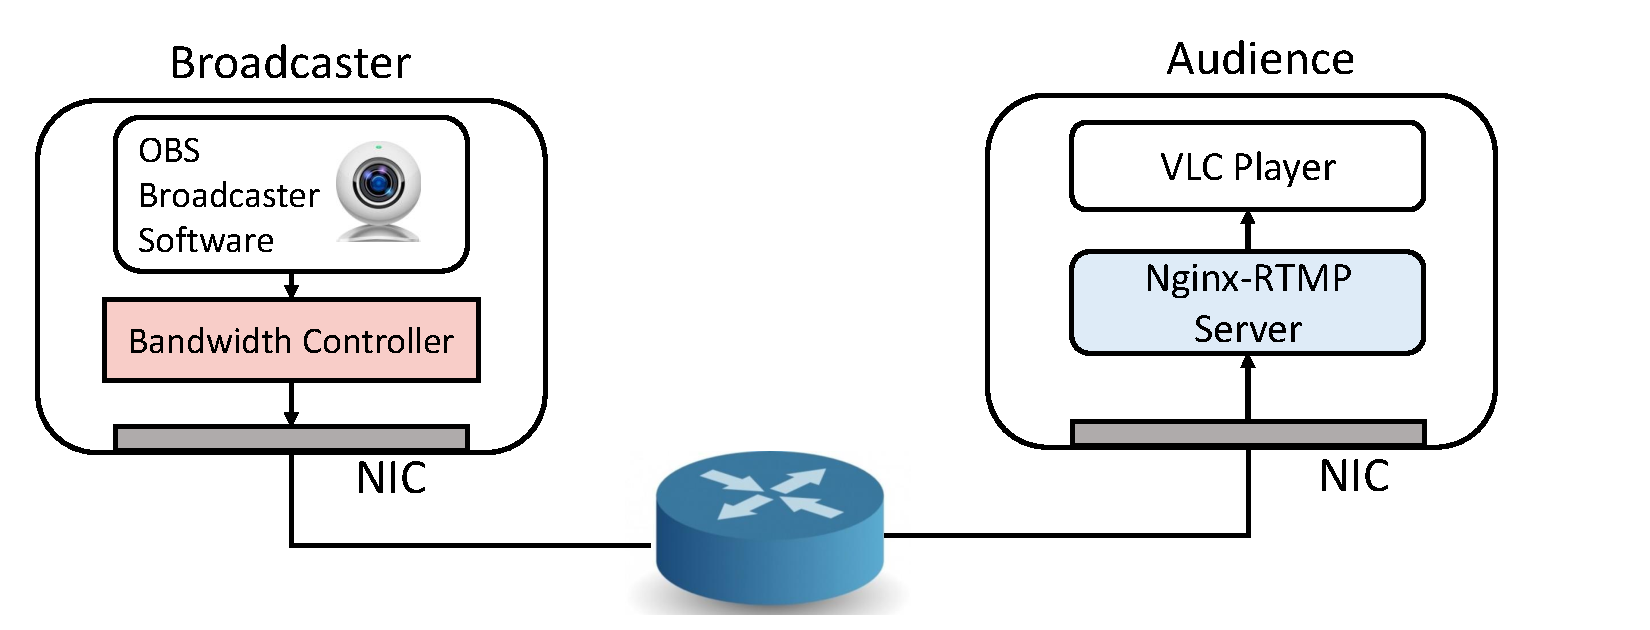
\includegraphics[width=\columnwidth]{fig/setup.pdf}
\caption{Experiment setup}
\vspace{-0.1in}
\label{fig:setup}\mylabel{fig:setup}
\end{figure} 
\textbf{Experiment setup.} We set up a live video streaming framework as in Figure~\ref{fig:setup}. The demo comprises of two modules, sender and receiver, which are connected by a switch in the middle. Servers both have 2 CPU cores and 6GB memory, and are equipped with $100$Mbps NICs. OBS studio\cite{OBS} is one popular broadcast software and is used to stream videos to the audience side over RTMP protocol in sender's side. We use both the tc module of linux and dummynet\cite{dummynet} to control the real-time upload bandwidth of sender. The broadcaster server(receiver) is built on nginx-rtmp module. On the audience server (receiver), VLC player is used to play the rtmp streaming.

%\begin{figure}[htb]
%\centering
%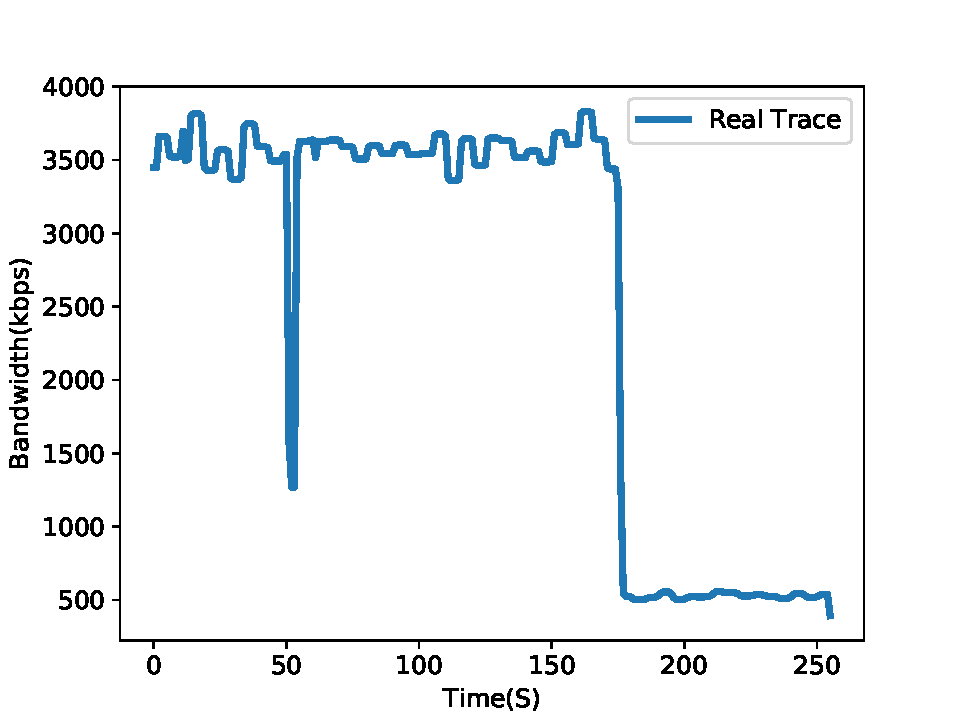
\includegraphics[width=.8\columnwidth]{fig/case_study_bandwidth.pdf}
%\caption{Bandwidth Control}
%\label{fig:case-bandwidth}\mylabel{fig:case-bandwidth}
%\end{figure}

\begin{figure}[htb]
\centering
\begin{subfigure}[b]{.45\columnwidth}
\centering
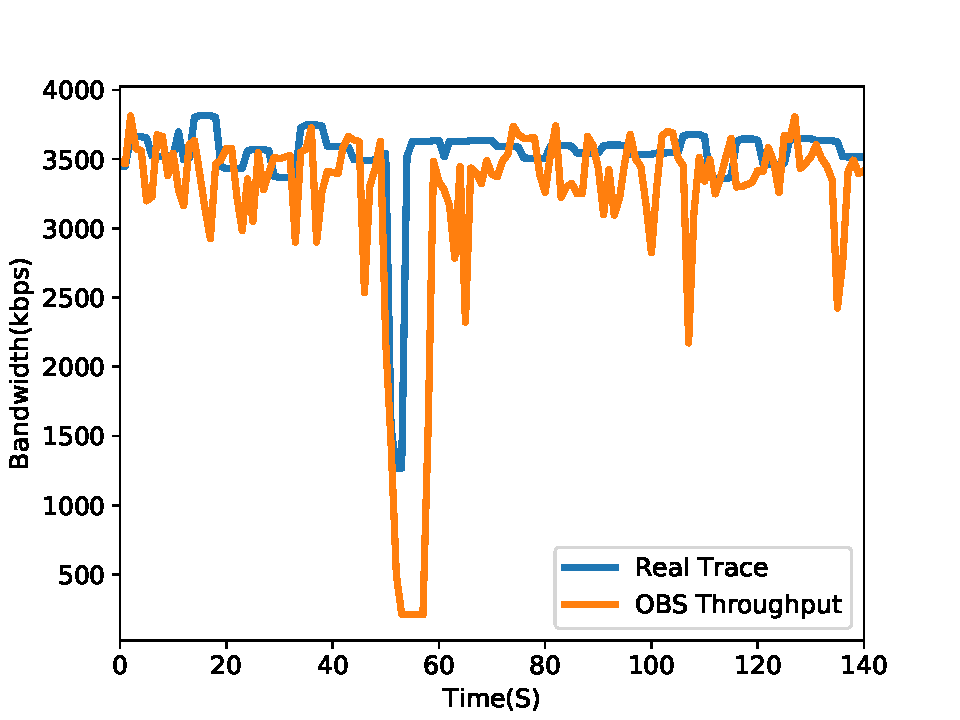
\includegraphics[width=\textwidth]{fig/case_study_throughput_a.pdf}
\caption{Throughput of $0-140$s}
\label{fig:case-throughput-a} \mylabel{fig:case-throughput-a}
\end{subfigure}
\begin{subfigure}[b]{.45\columnwidth}
\centering
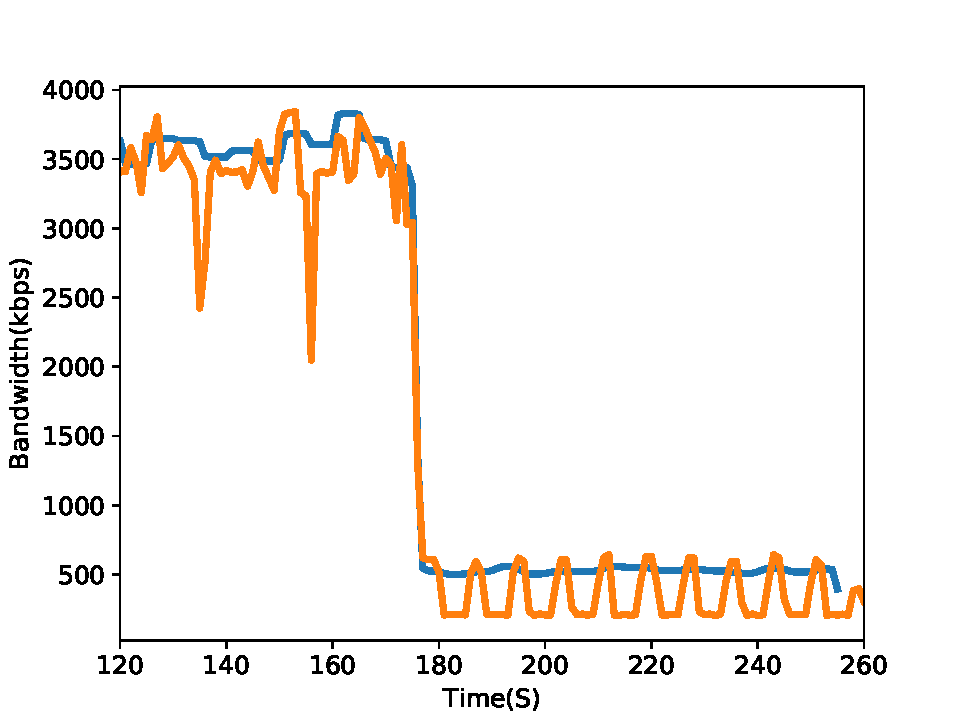
\includegraphics[width=\textwidth]{fig/case_study_throughput_b.pdf}
\caption{Throughput of $120-260$s}
\label{fig:case-throughput-b} \mylabel{fig:case-throughput-b}
\end{subfigure}
\caption{Case study: video streaming throughput in oscillating wireless network}
\label{fig:case-throughput} \mylabel{fig:case-throughput}
\end{figure} 
\textbf{Case study.} In the first motivating experiment, we control the network bandwidth according to an actual trace from a wireless network. The trace records the real-time network conditions when a user join the www.amazon.com on a mobile device. We aggregate packets in the trace into 5-second bins and calculate the data amount in each slot. We then control the network bandwidth on the sender side according to the per-second profile. The average bandwidth is up to $3000$kps, we stream video at a bitrate of $3000$kbps via OBS and capture actual video packet trace using tcpdump in the receiver's side. And the result is shown in Figure~\ref{fig:case-throughput}.  The trace lasts for $320$s, such a long time that we break the trace into two parts.

In the figure~\ref{fig:case-throughput-a}, the actual throughput follows the trace closely. However, at 50s, the network bandwidth falls below the bitrate and the situation lasts for 2 seconds, while the actual throughput degrades to almost zero from 50s to 58s. This is an abnormal behavior, as \textit{a 2-second network jitter cascadingly causes 8-second throughput falling in the streaming application.} Besides, a constant bitrate cannot efficiently handle long-term the bandwidth variance, which can be seen in Figure~\ref{fig:case-throughput-b}. Bandwidth is enough during $0-180s$, but after $180s$, the available bandwidth drops dramatically and lasts for $80s$, endless frames drop in this period. In this challenging network environment, the default OBS insists previous bitrate and obviously the strategy is not good.

\begin{figure}[htb]
\centering
\begin{subfigure}[b]{.45\columnwidth}
\centering
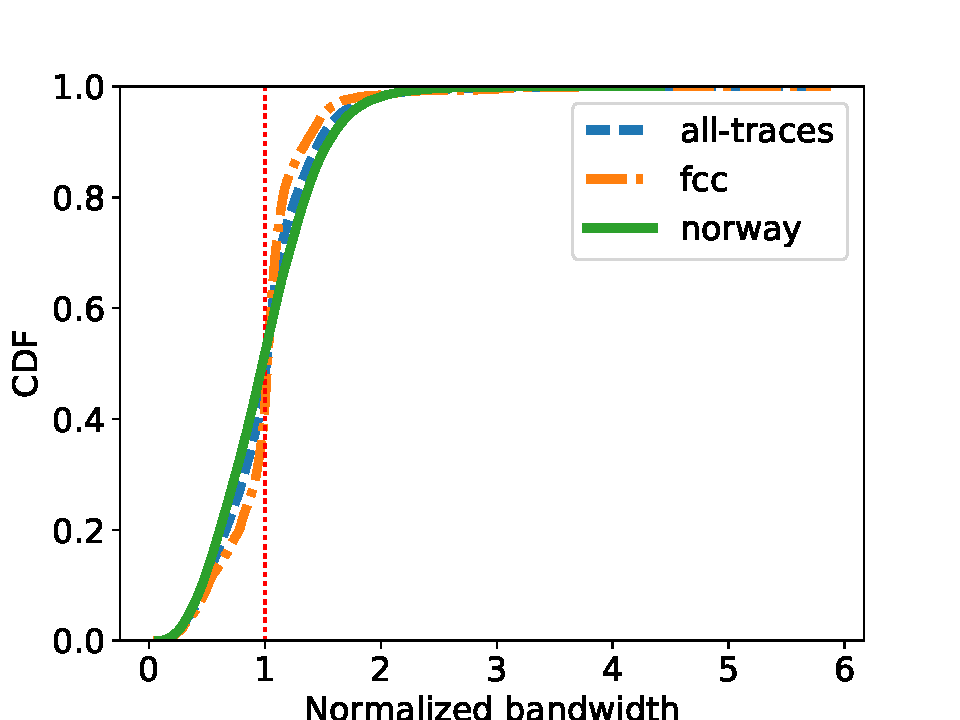
\includegraphics[width=\textwidth]{fig/trace.pdf}
\caption{Normalized Bandwidth}
\label{fig:trace}\mylabel{fig:trace}
\end{subfigure}
\begin{subfigure}[b]{.45\columnwidth}
\centering
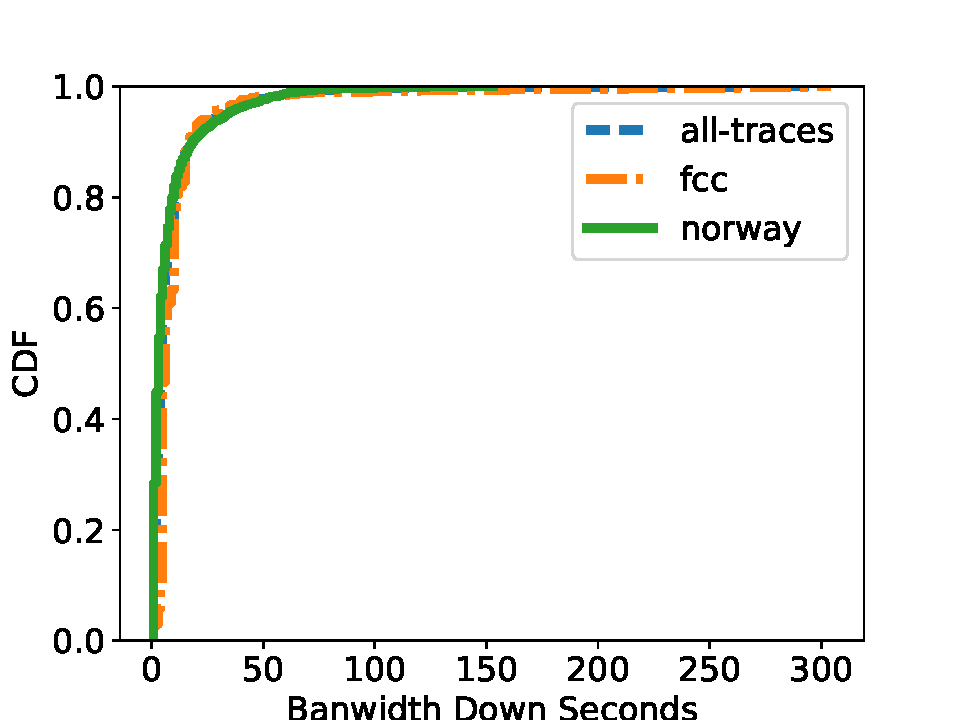
\includegraphics[width=\textwidth]{fig/trace-down.pdf}
\caption{Throughput Drop Time}
\label{fig:trace-down}\mylabel{fig:trace-down}
\end{subfigure}
\caption{Bandwidth distribution in wireless network}
\label{fig:trace-all}\mylabel{fig:trace-all}
\end{figure}

\textbf{Network Conditions} To know how often the bandwidth failure occurs, first we want to know the bandwidth distribution of real world. Two real-world dataset, FCC dataset\cite{FCC dataset} and HSDPA dataset\cite{HSDPA dataset}, is combined to calculate the bandwidth failure ratio. Each trace lasts for 320s, and the total dataset lasts for $30$ hours. For each trace, referring the average bandwidth as the unit, we normalize the trace and draw the cdf(Figure.~\ref{fig:trace}). Almost $50\%$ of traces are under the average throughput, which means for a $10$ second trace, about $5$ second the bandwidth is lower than the average. About $20\%$ of the traces are at most half of the average. The figure indicates that in real-time network, bandwidth fluctuation frequently occurs. To further explain how often long-term bandwidth fluctuation happens, we draw a picture of network failure time distribution, Figure~\ref{fig:trace-down}. Network failure time is calculated by counting the lasting time lower than the average bandwidth. About $20\%$ of the bandwidth fluctuation lasts for more than $10$ seconds, some even lasts for hundreds of seconds. Always using constant bitrate may introduce massive frame dropping.

\begin{figure*}[htb]
\begin{subfigure}[b]{0.32\textwidth}
  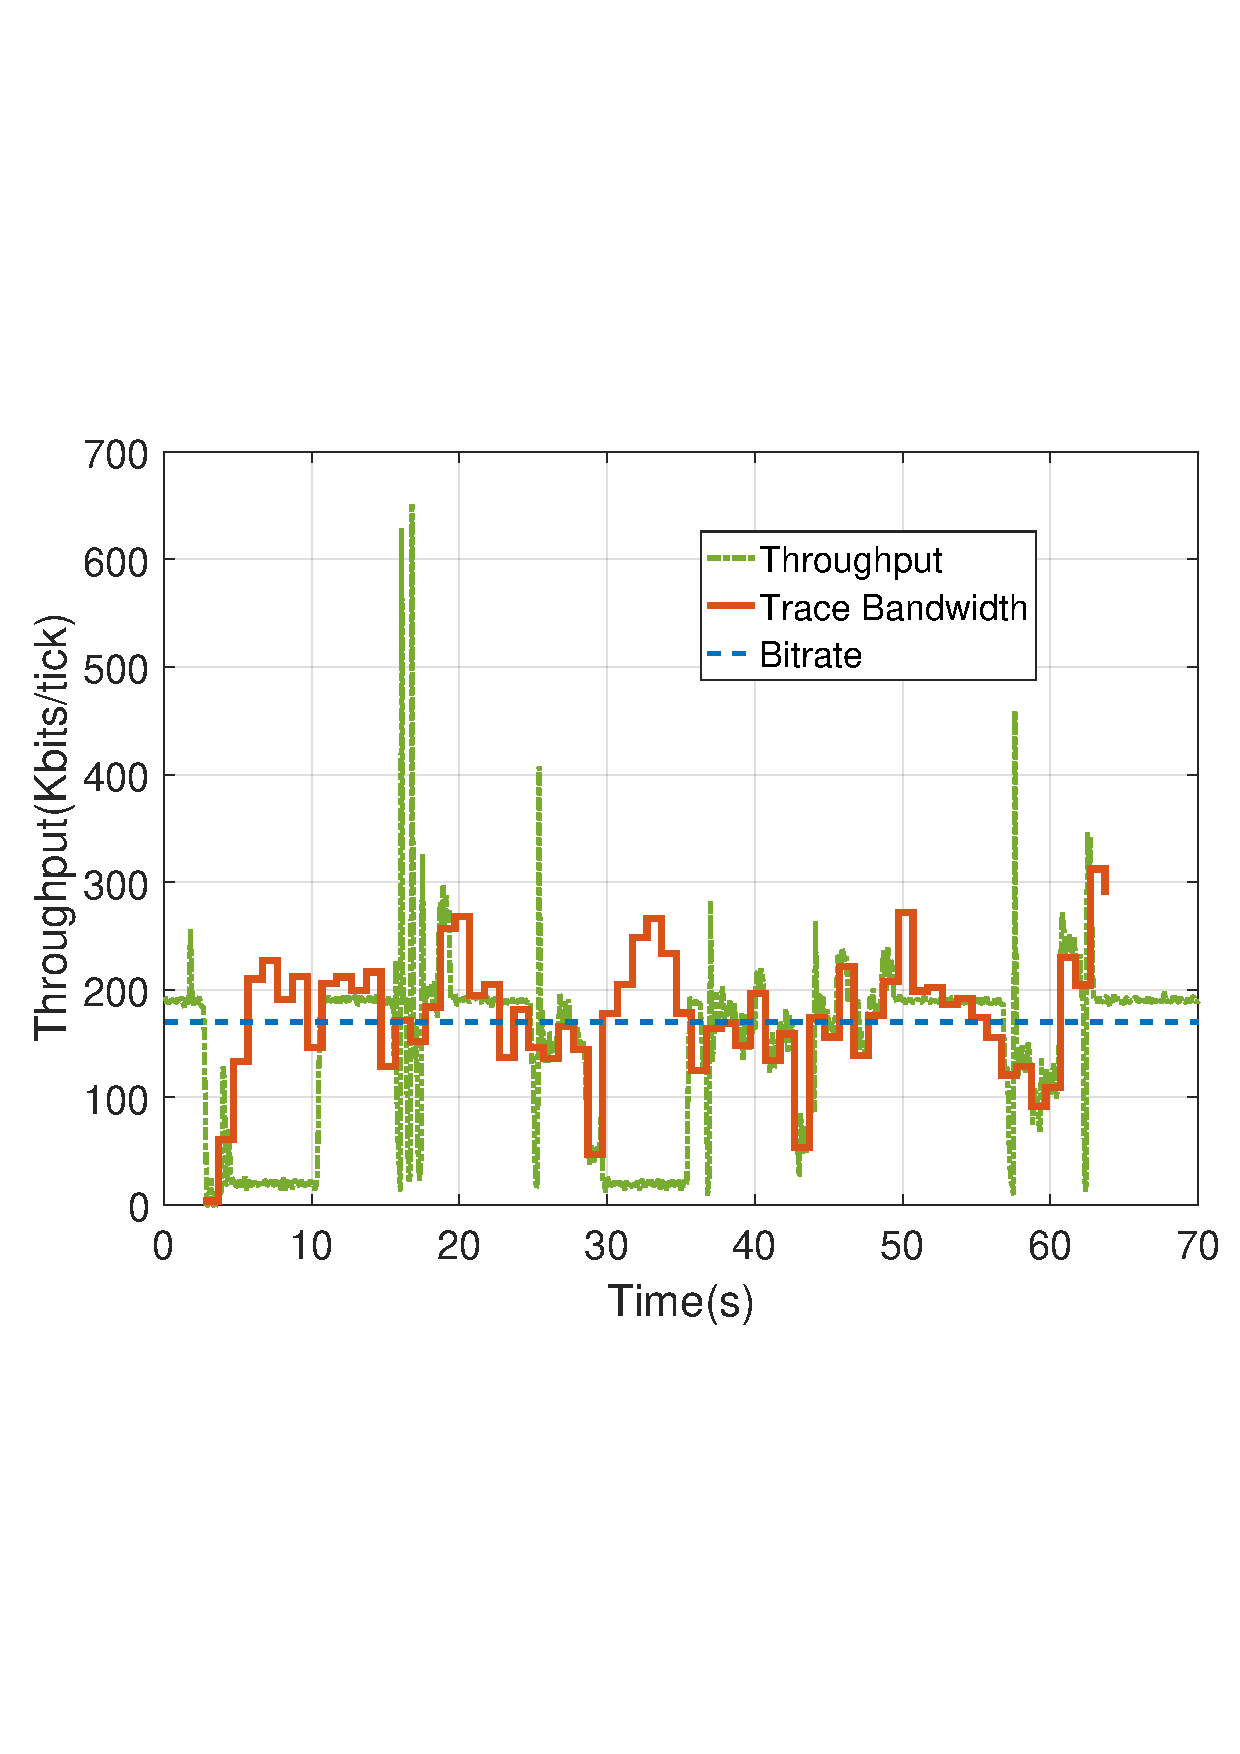
\includegraphics[width=0.8\linewidth]{fig/obs_douyu.pdf}
  \vspace{-0.05in}    
  \caption{OBS to Douyu server}
  \label{fig:obs-douyu}\mylabel{fig:obs-douyu}
\end{subfigure}
\begin{subfigure}[b]{0.32\textwidth}
  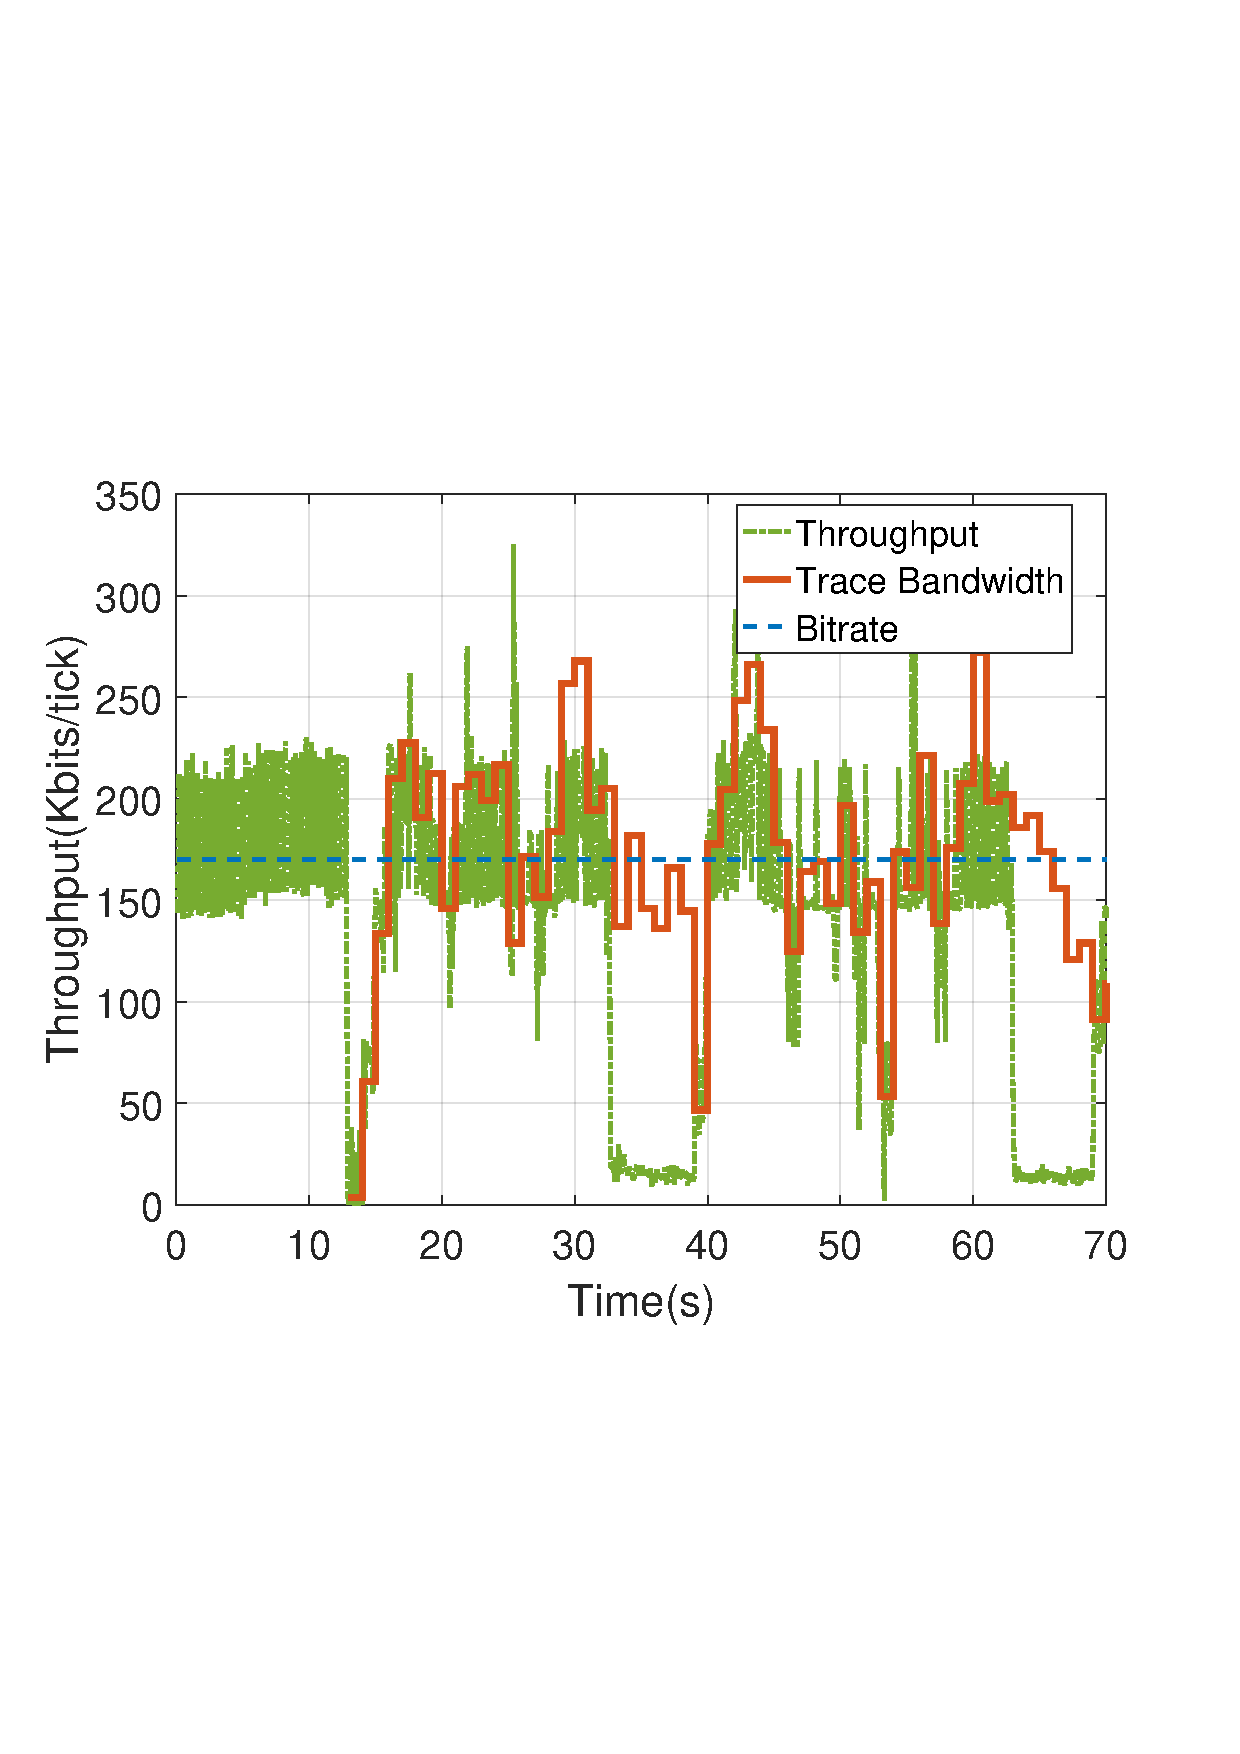
\includegraphics[width=0.8\linewidth]{fig/douyu.pdf}
  \vspace{-0.05in}    
  \caption{Douyu broadcaster to Douyu server}
  \label{fig:douyu}\mylabel{fig:douyu}
\end{subfigure}
\begin{subfigure}[b]{0.32\textwidth}%
  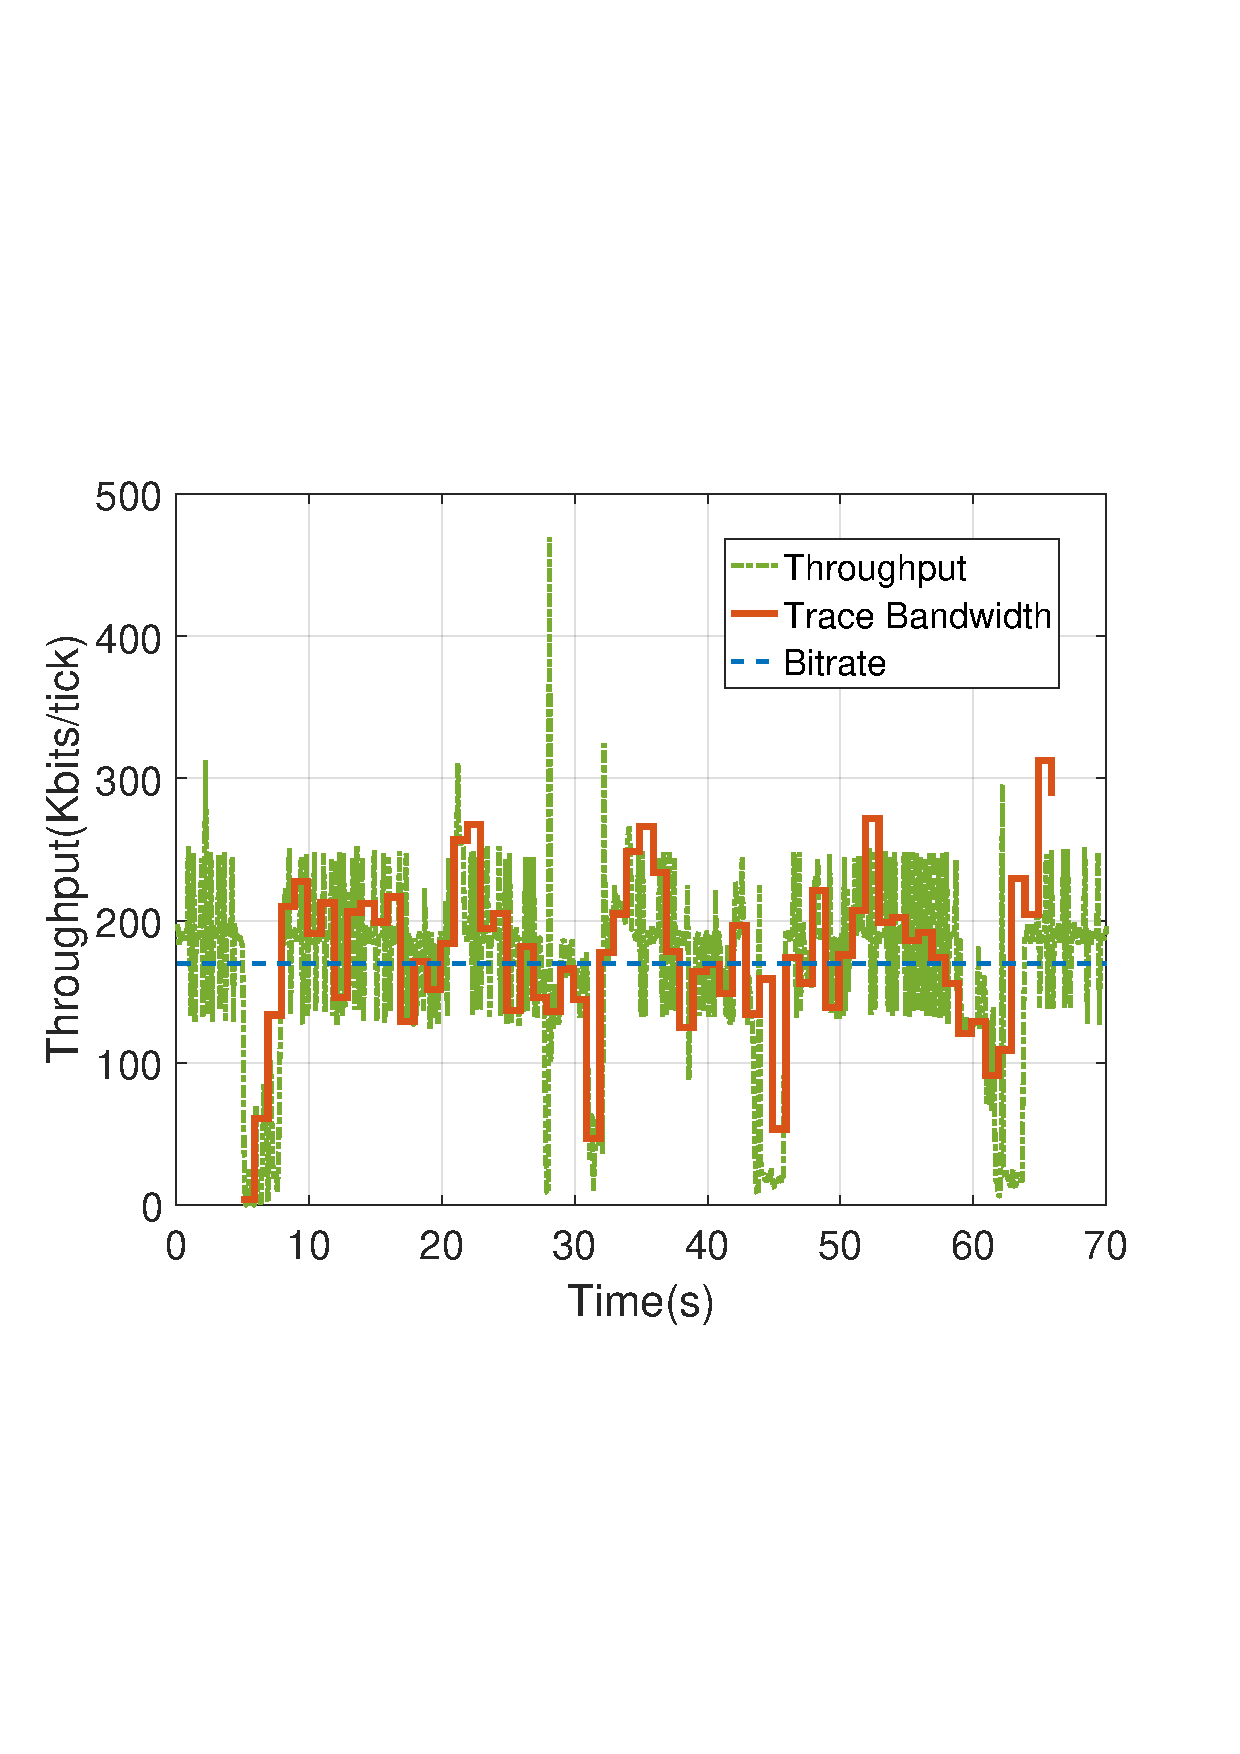
\includegraphics[width=0.8\linewidth]{fig/obs_twitch.pdf}
  \vspace{-0.05in}    
  \caption{OBS to Twitch server}
  \label{fig:obs-twitch}\mylabel{fig:obs-twitch}
\end{subfigure}
\caption{Throughput in three experiments}
\vspace{-0.15in}
\label{fig:commerical-throughput}
\end{figure*}

\begin{figure*}[htb]
\begin{subfigure}[b]{0.32\textwidth}
  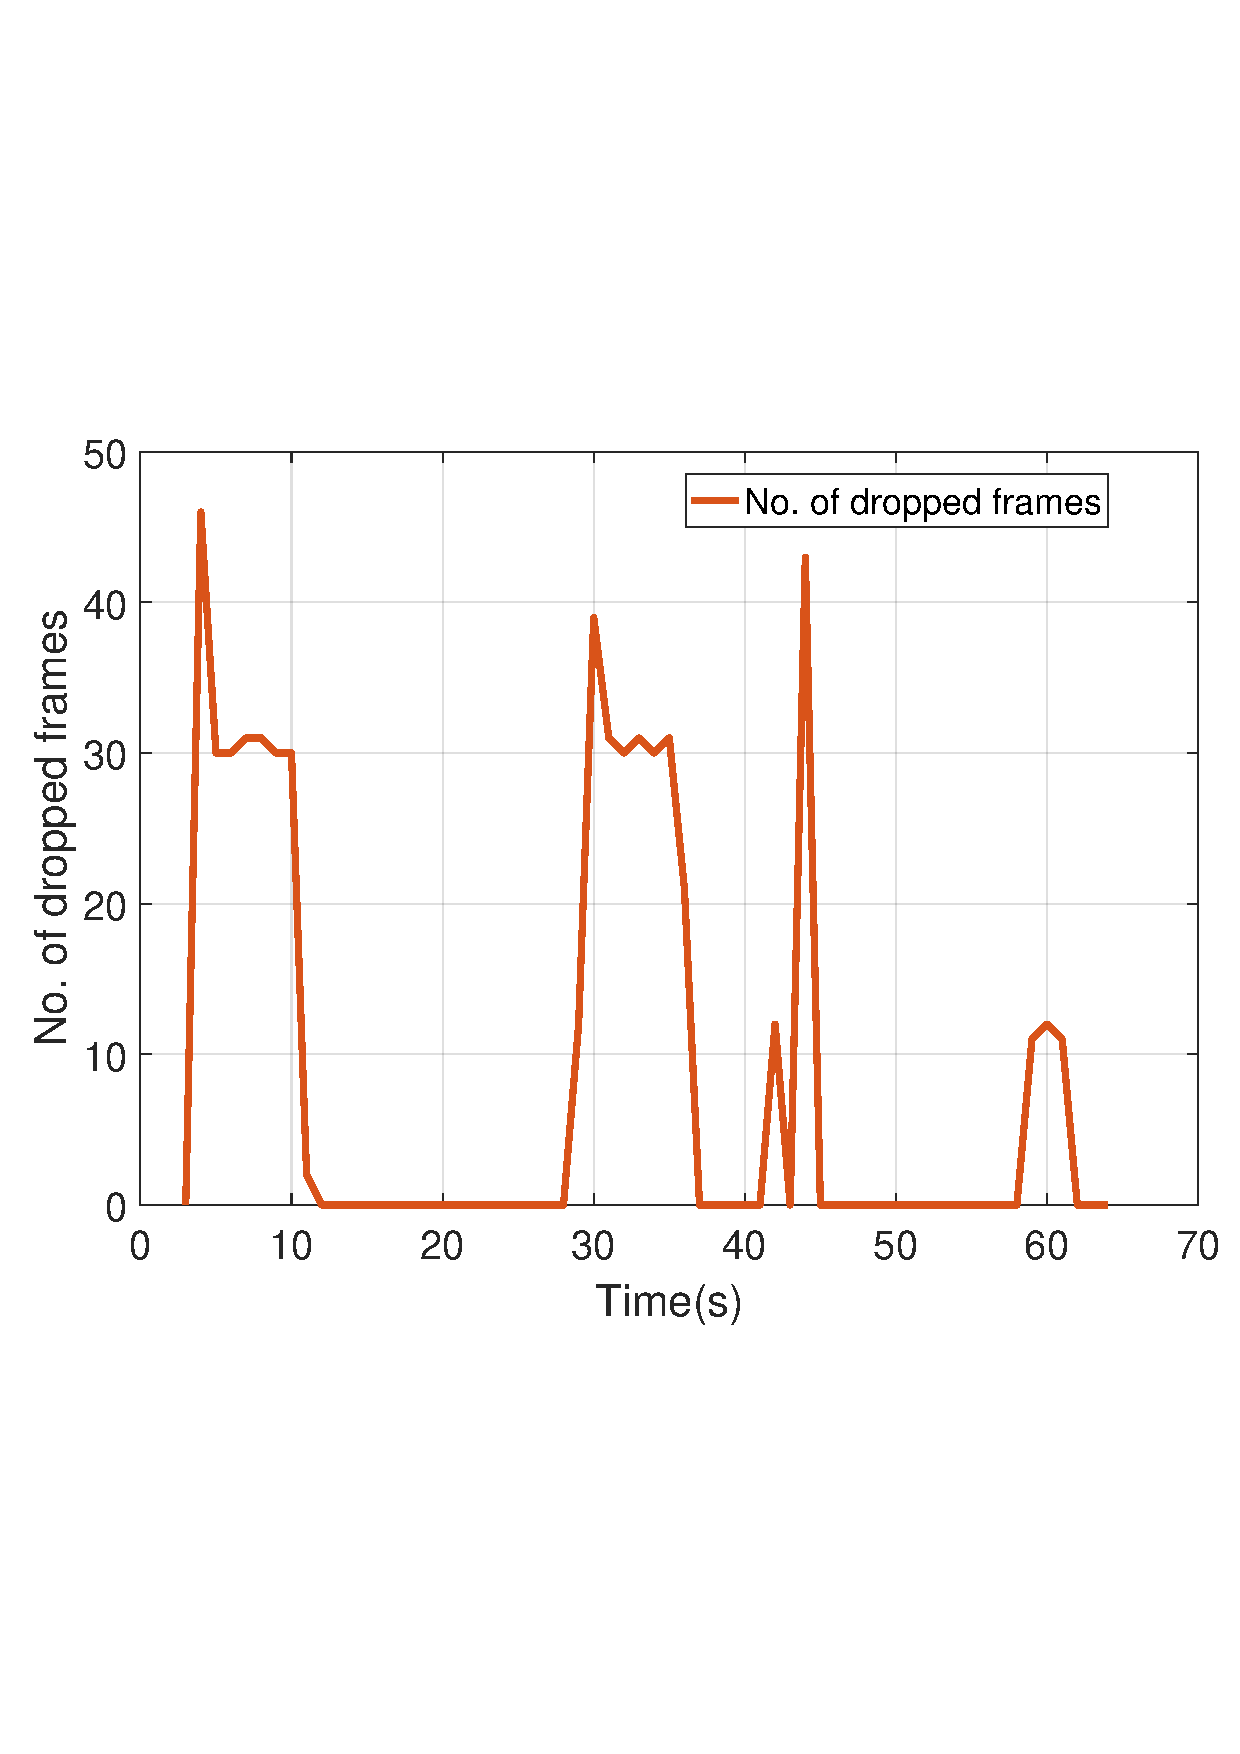
\includegraphics[width=0.8\linewidth]{fig/obs_douyu_drop.pdf}
  \vspace{-0.05in}  
  \caption{OBS to Douyu server}
  \label{fig:obs-douyu-drop}\mylabel{fig:obs-douyu-drop}
\end{subfigure}
\begin{subfigure}[b]{0.32\textwidth}
  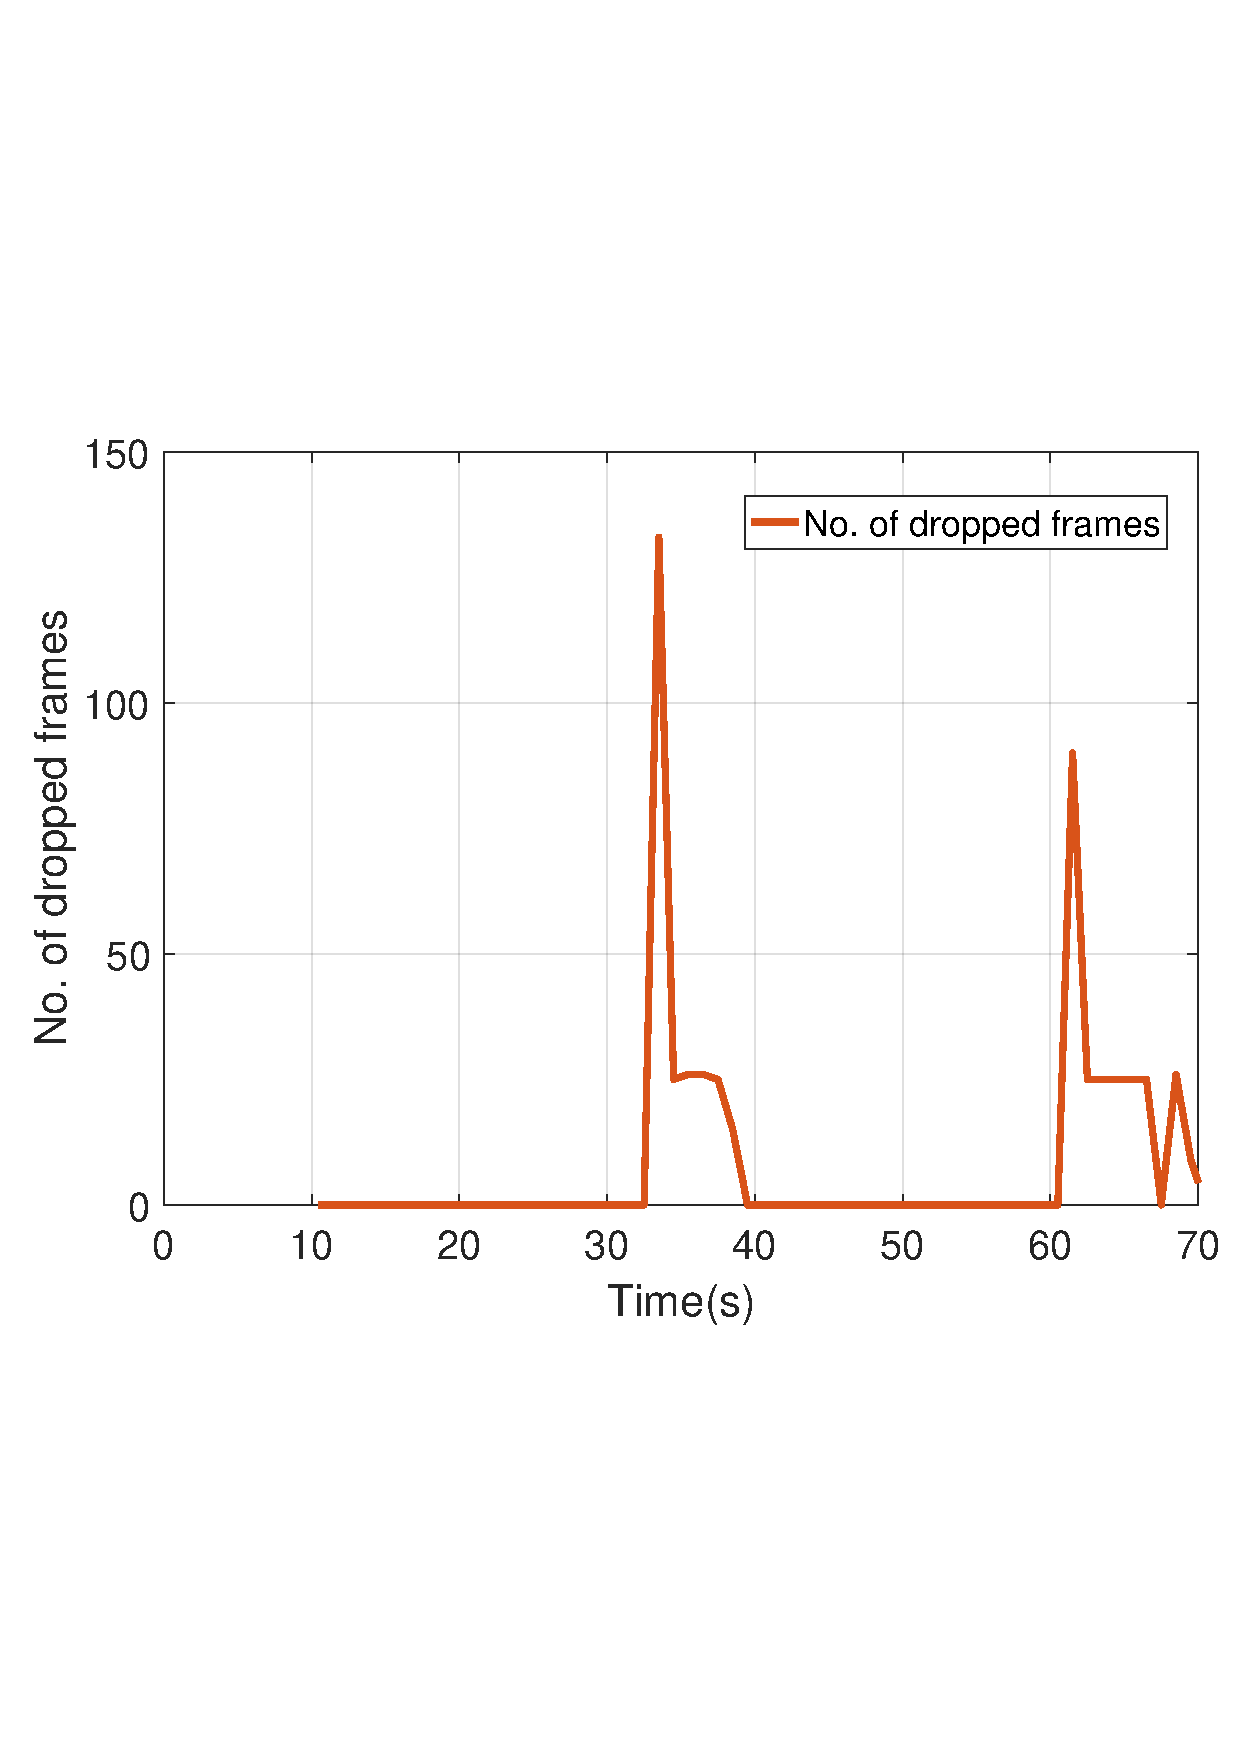
\includegraphics[width=0.8\linewidth]{fig/douyu_drop.pdf}
  \vspace{-0.05in}    
  \caption{Douyu broadcaster to Douyu server}
  \label{fig:douyu-drop}\mylabel{fig:douyu-drop}
\end{subfigure}
\begin{subfigure}[b]{0.32\textwidth}%
  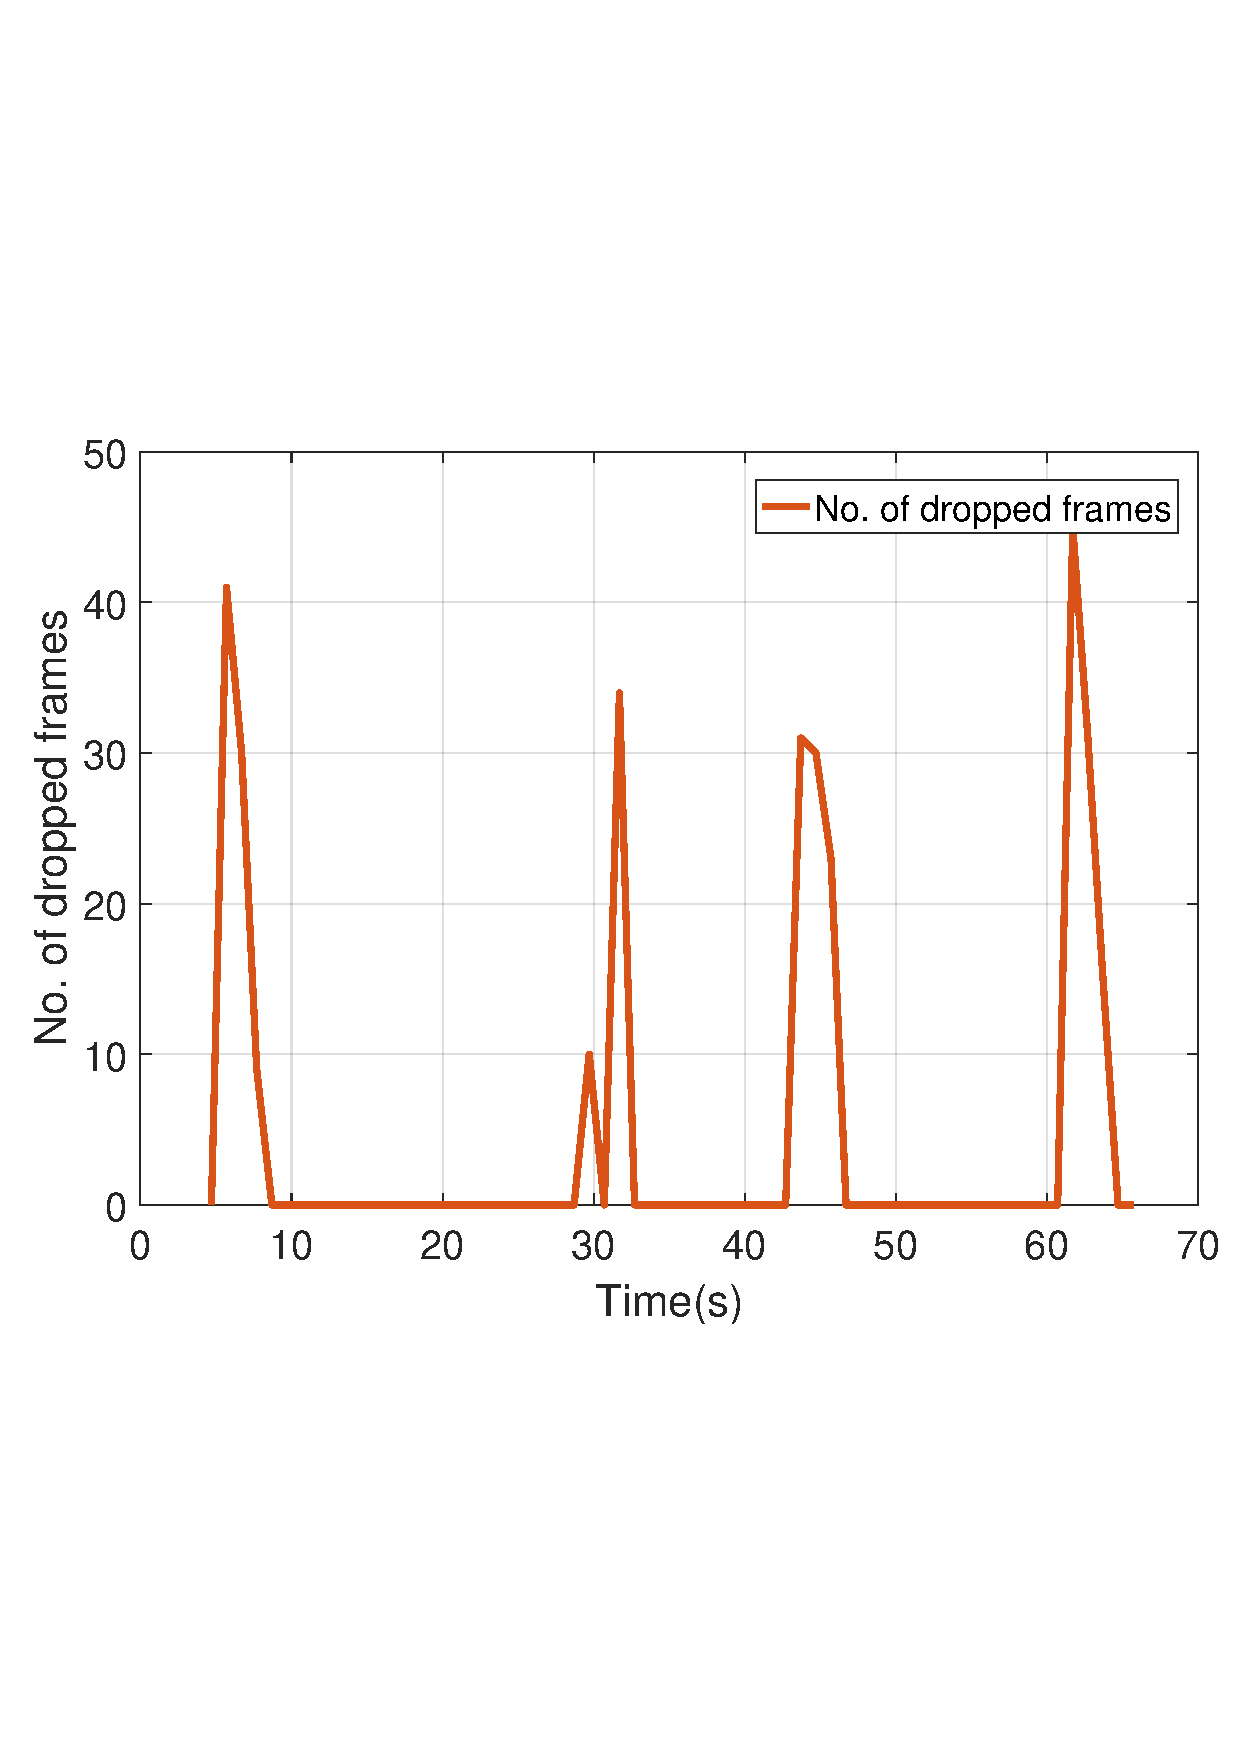
\includegraphics[width=0.8\linewidth]{fig/obs_twitch_drop.pdf}
  \vspace{-0.05in}    
  \caption{OBS to Twitch server}
  \label{fig:obs-twitch-drop}\mylabel{fig:obs-twitch-drop}
\end{subfigure}
\caption{No. of dropped frames}
\vspace{-0.2in}
\label{fig:commerical-drop}
\end{figure*}

\begin{figure}[htb]
\centering
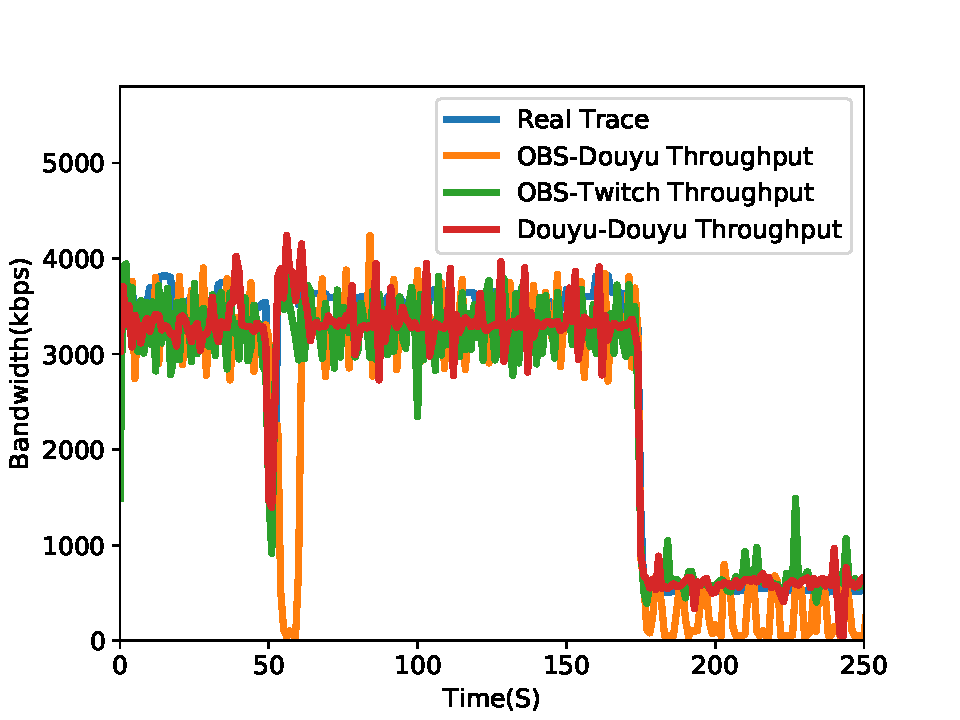
\includegraphics[width=.7\columnwidth]{fig/vary-bandwidth.pdf}
\vspace{-0.05in}
\caption{Throughput in long-time bandwidth drop case}
\vspace{-0.15in}
\label{fig:vary-bandwidth}\mylabel{fig:vary-bandwidth}
\end{figure}

\begin{table}[tb]
\centering
\caption{Frames dropped in different scenarios}
\label{tbl:drop}
{\setlength{\tabcolsep}{1pt}
\begin{tabular}{|c|c|c|l|}
\hline
\textbf{Experiment} & \textbf{Scenario} & \textbf{Play Failure(S)} & \textbf{ Failure Percentage(\%)}   \\ \hline
\multirow{3}{*}{Figure 5}&  Obs-douyu               & 18.1         & 30.2\%                           \\ \cline{2-4}
& Obs-twitch              & 9.9        & 16.3\%    \\ \cline{2-4}
& Douyu-douyu            & 16.6      & 27.2\% \\ \hline
\multirow{4}{*}{Figure 7} & Obs-douyu            & 93.1      & 37.2\%     \\ \cline{2-4}
& Obs-twich             & 79.3      & 31.7\%  \\ \cline{2-4}
& Douyu-douyu             & 66.67         & 26.7\%  \\ \hline
\end{tabular}}
\vspace{-0.2in}
\end{table} 
\textbf{Experiments on several commercial platforms.} We further repeat the experiment in different commercial platforms and settings to find whether the same issues exists. We test three different situations, including OBS pushing video to Douyu server, Douyu broadcaster to Douyu server, and OBS to twitch server. In three experiments, the bitrate is choose lower than the average bandwidth, $1700$kbps. Tcpdump is used to record the real-time throughput, we aggregate the data size in one tick(0.1s) together and draw a picture.
Figure~\ref{fig:obs-douyu}, ~\ref{fig:douyu}, and~\ref{fig:obs-twitch} show the throughput of the three experiments respectively, Figure~\ref{fig:obs-douyu-drop}, ~\ref{fig:douyu-drop}, ~\ref{fig:obs-twitch-drop} is the corresponding number of dropped frames. The first three lines in Table~\ref{tbl:drop} show the total frame drops during the experiment.

Comparing the results across different platforms, we observe that the ``cascading effect'' is prevalent, appearing on all platforms (e.g., the 30s in OBS to Douyu, the 32s in Douyu to Douyu, and 43s in OBS to Twitch). For these three time period, the frame dropping keeps a high value. We also find out that the cascading effect is not related to the instantaneously available bandwidth. For example, in Figure~\ref{fig:obs-douyu}, a dramatic bandwidth drop at 30s causes the cascading frame drop; while in Figure~\ref{fig:douyu}, a slight bandwidth drop at 32s causes the frame drop. Another observation is that the length of the cascading drop is different on different platforms: $5+$s in Douyu and 2-3s in Twitch. Finally, from Figure, we observe that the broadcaster software usually can tolerate short-period throughput drop without dropping frames, but cannot tolerate long-period ones.

\subsection{Analyzing the Root Cause}
\begin{figure}[t]
\centering

\includegraphics[width=0.9\columnwidth]{fig/drop.pdf}
\vspace{-0.08in}
\caption{Producer-consumer model of streamer's buffer}
\vspace{-0.1in}
\label{fig_drop}
\end{figure} 
%\wenfei{1. decoding sequence, 2. consumer-producer mode, 3. cascading effect.}

The cause of ``frame drop'' is the buffer management in the streaming software. There exists a queue to temporarily store video frames; a video frame generating thread captures images from the camera, encodes raw images into H.264 frames, and enqueues the H.264 frames; while a frame sending thread dequeues frames and send them to the network via TCP socket operations (e.g., \mywrite).
%The two threads form a typical consumer-producer model.
If the network is in bad conditions, the frame sending thread would be blocked, and then the queue accumulates until a threshold, causing the frame generating thread unable to enqueue frames and thus dropping them.
\begin{figure}
\centering
%\small
{\setlength{\tabcolsep}{3pt}
\begin{tabular}{|r||ccccccccc|cc|}
\hline
Frames                                                       & I & B & B & P & B & B & P & B & B  & I  & ... \\ \hline
Display order                                                & 1 & 2 & 3 & 4 & 5 & 6 & 7 & 8 & 9  & 10 & ... \\ \hline
Coding order & 1 & 3 & 4 & 2 & 6 & 7 & 5 & 9 & 10 & 8  & ... \\
\hline
\end{tabular}}
\caption{H.264 frame display/coding order}
\vspace{-0.3in}
\label{fig:frame-order}\mylabel{fig:frame-order}
\end{figure}
\begin{algorithm}[tb]
\caption{OBS Frame Enqueue Management}
\label{alg:obs-drop}\mylabel{alg:obs-drop}
\begin{algorithmic}[1]
\State \textbf{Input:} frame
\State T1 := 0.9s, T2 := 0.7s
\If{frame is I frame}
\State dropPFrame := False, dropBFrame := False
\State \Call{Enqueue}{queue, frame}, \Return
\Else
\State timespan := \Call{TimeSpan}{queue}
\EndIf
\If{frame is P frame}
\If{dropPFrame or timespan $>$ T1}
\State \Call{Drop}{frame}, \Call{Drop}{queue, `P'}
\State dropPFrame := True
\Else
\State \Call{Enqueue}{queue, frame}
\EndIf
\ElsIf{frame is B frame}
\If{dropBFrame or timespan $>$ T2}
\State \Call{Drop}{frame}, \Call{Drop}{queue, `B'}
\State dropBFrame := True
\Else
\State \Call{Enqueue}{queue, frame}
\EndIf
\EndIf
\end{algorithmic}
\end{algorithm} 

The cause of the ``cascading'' drop is the dependency between frames. In H.264, a piece of video is organized into groups of pictures (GOP). During the encoding, the first frame in each group is kept unchanged (I frame); a few P frames are generated by computing their delta with the preceding I or P frame; a B frame is computed based on its neighboring I and/or P frames. Figure~\ref{fig:frame-order} shows an example of a series of I, B, P frames. The frames are indexed by display order, but the encoding/decoding is in a different order according to the dependency. Due to the dependency, when a P frame in the middle of a GOP is dropped, all following P, B frames within the same group would not be able to decode. Thus, if a small interruption from the network causes frame drop in the beginning or middle of a group, it cascading causes the remaining frames in the same group not decodable (or simply dropped).

We studied OBS broadcaster software and list its frame management algorithm (Algorithm~\ref{alg:obs-drop}). At first, the drop priority are set to false. When a new frame arrives at the queue, if it is I frame, it is enqueued (never dropped); otherwise, the timespan of the frames in the queue is computed (i.e., the difference of the display timestamps between the latest and the earliest frame). If the incoming frame is a P frame, and if the timespan is smaller than 0.9 second, the P frame is enqueued; but if the drop priority corresponding P frame is true, the P frame is dropped; and if timespan is larger than 0.9 second, all P and B frames (including the ones in the queue and incoming ones) within the GOP are dropped, all the drop priority are set to true. Similarly, if the incoming frame is a B frame, the threshold is 0.7 second, and the processing logic is the same with that of P frames.

\iffalse

The broadcaster usually runs software from the platform provider to generate live video and upload it an RTMP server. We studied an existing commercial video streaming software OBS~\ref{XX}; it has a video frame generating thread and frame sending thread, which forms a typical consumer-producer model. The video frame generating thread capture raw images from the device camera and encoding them into video frames (e.g., H.264), and enqueue the generated frames into a queue. While the frame sending thread takes frames from the queue and calls TCP socket interface (\mywrite) to send frames into the network. If the network is in bad conditions, the sending thread is blocked by the \mywrite operation of TCP, and the queue accumulates until a threshold causing the frame generating thread to drop frames.


There exists three kinds of frames, 'I', 'P', 'B', in H.264 format. 'I' frames are independent, 'P' frames depend on previous 'I' or 'P' frames. 'B' frames depend on neighbouring 'I', or 'P' frames. Missing higher priority frames will lead to decoding error to lower priority frames.
Streamer usually maintains a shallow buffer, as the figure shows\ref{fig_drop}. Encoder pushes the encoded frames into the buffer, at the same time, the streamer popes the buffered frames into the TCP socket. Reading the source code of OBS, we find that the default strategy results in the quality issue. Default strategy goes like that, record the time length of buffered frames, if the time larger than a certain value $0.7s$, drop all the B frames in the buffer, and reject all the following B frames until a P frame arrive. If the buffer exceeds $0.9s$, drop all the P frames in the buffer and to come, and wait for the key I frame. Dropping one P frame means all the remaining P frames in the GOP is useless, and a GOP usually lasts for a few seconds(for example, default 9s in OBS). Dependency of different frames and dropping frames lead to such quality issue.

H.264 is the typical video encoding mechanism using in video streaming. To generate video in the format of H.264, raw frames are put into groups of pictures (GOP), and then H.264 frames are computed within each group. In each group, the first frame is kept as I frame without change; a few P frames are computed by computing their delta with the preceding I frame or P frame; a B frame is computed based on its neighboring I frame and/or P frames. In video streaming, the broadcaster can preconfigure several parameters, including frames per second (FPS), resolution (width and height), and bitrate. During the video compression from raw frames to H.264 frames, I, P, B frames are computed and filters may be used to keep the preconfigured bitrate. For example, if the bitrate is low and FPS and resolution are high in the configuration, then the video compression filter would generate ``big pixels'' to reduce the bitrate, which actually reduce the video quality.

Combining the I, P, B frame in H.264 and the queue management in OBS, we present its frame dropping strategy. The frame sending thread always tries its best to dequeue and send frames. In the frame generating thread, I frames are always enqueued without dropping; for an incoming P frame, if the most recent frame in the queue is 0.9 second later than the most recent frame, the current P frame and existing P frames in the queue is dropped, and otherwise the P frame is enqueued; similarly for B frames, the threshold is 0.7 second.


Combining these two requirements, we find naive solutions is hard to guarantee both of them. To make the streaming resistant to bad network conditions such as low throughput and occasional jitters, the broadcast software tends to have larger buffer/queue to hold frames when the network cannot send them; while larger buffer would cause larger queuing delay, which hampers the requirement of low latency. Thus, we believe it is unique and challenging to achieve low-latency user-generated live video streaming that is resistant to unstable

\fi

\iffalse
\subsection{Commercial Applications}
To validate whether the commercial service provider has solved the issue, we repeat the same black box experiment on two commercial platforms(Twitch, Douyu) and three streamer(OBS, Douyu Tools, XSplit) respectively.
\fi

%%\section{A closer look at the quality issues}

\iffalse

We set up a live video streaming framework as in figure. The streamer side equipped with one network interface card(NIC) sends a video streaming to the server. The server is build on nginx-rtmp module to support RTMP protocol. We use VLC player to supervise the video streaming at the server side, and use tc to control the latency, bandwidth of the link.

In the example experiment, we set the streaming bitrate to be $2000$ kbps, a value that frequently adopted, the link condition varies according to real-world data trace \cite{iitkgp-apptraffic-20151126}, and capture the packet trace using Wireshark. Figure \ref{fig_trace} shows the packet trace. We aggregate packets into $100$-ms intervals and count the throughput in each interval. The x-axis shows time elapsing during the measurement, and the y-axis shows the throughput in each interval.

\begin{figure}[t]
\centering
\includegraphics[width=0.9\columnwidth]{Throughput.pdf}
\vspace{-0.08in}
\caption{Packet trace in the experiment}
\vspace{-0.1in}
\label{fig_trace}
\end{figure}

Before $80$s, the throughput in each $100$-ms interval roughly equals to the regular value. But at $80$s, the throughput experiences a period of almost-zero, after several seconds, the throughput returns normally. At the strange period, we observe buffering and black screen in server side

\subsection{Key Factors}
We do some controlled experiments, using the open source live streaming software, OBS, to further explore the root cause.
\subsubsection{Different Starting Time}
We set the bitrate to $2000$ kbps, the keyframe interval to $8$s and other parameters to default value. We observe that for different starting time, even for the same interruption time, the number of dropped frames differs greatly, Fig. \ref{fig_starttime}. We take the starting time [17,19,21,23] as example, the number of dropped frames has a linear relationship with the starting time. Another interesting finding is that the number of dropped frames displays a regular pattern every $8$s, which is exactly the keyframe interval \ref{tab_startregular}.
\begin{figure}[t]
\centering
\includegraphics[width=0.9\columnwidth]{StartTime.pdf}
\vspace{-0.08in}
\caption{Number of Dropped Frames for Different Start Time}
\vspace{-0.1in}
\label{fig_starttime}
\end{figure}

\begin{table}[!htb]
\centering
\caption{Number of Dropped Frames for Different Start Time}
\label{tab_startregular}
\begin{tabular}{|l|l|l|l|l|}
\hline
Starting time(s)       & 9     & 17    & 25    & 33  \\ \hline
Average Dropped Frames & 202.2 & 203.8 & 198.6 & 199 \\ \hline
\end{tabular}
\end{table}


\subsubsection{Network Interruption Time}


\subsubsection{Video Bitrate}
We choose the streaming video bitrate set to $[1000,1500,2000,2500]$ kbps, and the measurement results are as follows\ref{tab_Bitrate}.
The network is controlled to cut off at $19$s, and recover at $21$s. Keyframe interval is $8$s by default.
For these different video bitrates, the number of dropped frames seems all the same. Given enough bandwidth, changing the video bitrate wouldn't make any difference. Dropping frame strategy has no relationship with streaming bitrate.
\begin{table}[!htb]
\centering
\caption{No. of Dropped Frames}
\label{tab_Bitrate}
\begin{tabular}{|l|l|l|l|l|}
\hline
Bitrate(kbps)          & 1000  & 1500  & 2000  & 2500  \\ \hline
Average Dropped Frames & 148.2 & 148.2 & 149.0 & 150.6 \\ \hline
\end{tabular}
\end{table}

Frame dropping mainly depends on three factors: (1)starting time (2) interruption time.

\subsection{Design space}

\fi

%\section{A closer look at the quality issues}
\subsection{Design Space Insight}
To meet the delay constraints, there are two kinds of solution. One is to limit the timeliness of the sender buffer, strictly restrain each frame to meet the time requirements; the other maybe controlled by scheduling to maintain the average of delay at the target value, this is . In our case, the first one is our choice. We limit the buffer size to $0.9s$.

With buffer size limited, the previous motivating example gives us three intuitions to improve the video streaming quality.
\textbf{Eliminate the dependency between frames.}
By this means, the solution space would be larger and more optimal solutions are expected to be found.

There are two ways to implement this constraint relaxation. A naive approach is to reduce the keyframe interval. For example, if a 2-second interruption starts at the beginning of an 8-second GOP, the whole group are dropped; but if the 8-second GOP is refined to be four 2-second GOP, only one 2-second GOP would be dropped. Thus, the cascading effect would be eliminated. However, this approach may be a tradeoff between the minimal frame drop and the video quality, because reducing keyframe interval means less compression in video streaming, to keep a pre-configured bitrate, per-image quality would be degraded (i.e., ``big pixels''). The method needs a good tradeoff between video quality and frame dropping.

Another approach is to make the GOP selection adapt to the network condition. In details, when the network recovers from an interruption, the first frame transmitted is encoded as I frame, and a new GOP restarts from this first frame. In this way, the new GOP has no dependency with previous (possible dropped) frames, and all its frames are decodable. This approach may need to modify the encoding workflow, which is hard and out of control.

\textbf{Improve the frame drop strategy.} The default strategy in OBS is dropping all P/B frames in buffer when exceeding a threshold. It's some reasonable because if dropping the earlier frames, the following frames cannot be decodable; and if dropping the latest several frames, the earlier frames still exist in buffer, the timeliness will be violated. But intuitively, dropping frames within the old GoP, rather than all, may have better performance. It is worth thinking how to design an online frame dropping strategy that approaches the optimal solution. The challenge lies in the complexity of the frame dependency. A brute force solution is impossible due to its time complexity.

\textbf{Adaptive bitrate.} Network failure occurs frequently. Conclusions from figure~\ref{fig:trace-all} validate the fact. Measurements show that commercial applications only use constant bitrate(CBR) or ABR, which means the actual bitrate varies among the target value, at most $20\%$ lower or higher of the target bitrate. These two methods cannot follow the changing bandwidth, which would bring tremendous frame dropping when bandwidth falls down. Especially in the case where the bandwidth drop lasts for a certain while. One possible solution is similar with DASH in VOD scenario, applying adaptive bitrate in broadcaster's side. In our case, the bitrate differs between two GoPs, which means we would decide a bitrate for each GoP. Introducing bitrate adaptation maybe dramatically cut down the frame dropping.

\iffalse
\begin{itemize}
\item If we can relax the dependency between frames, the solution space would be larger and more optimal solutions are expected to be found. That is, we can relax the decodability constraints to be $d_i = 1, \forall i$.

\item We can relax queue length constraint, i.e., making $T_1$ larger. This change similarly increases the space of possible solutions.

\item The frame drop strategy can be improved. That is, compared with the naive strategy in OBS (dropping all P/B when exceeding a threshold), selectively choosing frames to drop in IP would give a more optimal solution.
\end{itemize}
\fi


\newcommand{\Mod}[1]{\text{ (mod } #1\text{)}}
\wenfei{edit until here. would come back at 2PM}
\section{Our Solution}
In this section, we present GVBR, a suite of techniques built on the
aforementioned design principles to optimize personalized live streaming
quality.
In particular, GVBR optimizes the adaptation at frame-level
(Section~\ref{subsec:drop-strategy}), as well as GOP-level
(Section~\ref{subsec:adaptive-bitrate}).

\subsection{Drop Strategy}
\label{subsec:drop-strategy}
\subsubsection{Problem Formulation}
\begin{table}[tb]
\footnotesize
\centering
\caption{Terminology in Integer Program}
\label{tbl:term}
{\setlength{\tabcolsep}{1pt}
\begin{tabular}{|c|c|l|}
\hline
\textbf{Symbol} & \textbf{Type} & \textbf{Meaning}                      \\ \hline
$i$               & index         & frame index                           \\ \hline
$j$               & index         & time index                            \\ \hline
$x_{ij}$             & variable      & whether frame $i$ is in queue at time $j$ \\ \hline
$y_{ij}$             & variable      & whether frame $i$ is sent at time $j$     \\ \hline
$z_{ij}$             & variable      & whether frame $i$ is dropped at time $j$  \\ \hline
$T$               & const         & decision time                        \\ \hline
$T_1$             & const       & max time when a frame keeps ``fresh'' \\ \hline
$C_j$              & const         & network bandwidth at time $j$           \\ \hline
$N$               & const         & key frame interval                      \\ \hline
$S$            & const         & each frame size                        \\ \hline
$M_{j}$       & const         & frame index that can be send at time $j$ \\ \hline
$R_{i}$        & const         & bitrate of the $i$ frame               \\ \hline
\end{tabular}}
\end{table}

\begin{figure}[tb]
\centering
{\setlength{\tabcolsep}{3pt}
\begin{tabular}{|l|l|}
\hline
\multicolumn{2}{|c|}{ maximize $\Sigma_i y_{iT}$, subject to} \\ \hline \hline
 $x_{ij}+y_{ij}+z_{ij} = 0, \forall j<i$       & (1)        \\
 $x_{ij}+y_{ij}+z_{ij} = 1, \forall j\geq i$   & (2)       \\
 $x_{ij} \geq x_{i,j+1}, \forall j\geq i$      & (3)        \\
 $y_{ij} \leq y_{i,j+1}, \forall j\geq i$      & (4)        \\
 $z_{ij} \leq z_{i,j+1}, \forall j\geq i$      & (5)        \\ \hline
 $y_{ij} = \max\{1,{1-z_{i,j-1}}\}, \forall j, i \leq M_{j}$  & (6)   \\ \hline
 $y_{ij}+z_{ij} = 1 ,\forall j>i+T_2$          & (7)        \\ \hline
 $y_{i+1,T} \geq y_{iT}, \forall i \not\equiv N-1 (\text{mod}N)$ &(8) \\ \hline
\end{tabular}}
\caption{Frame Drop Strategy}
\label{fig:ip-program} \mylabel{fig:ip-program}
\end{figure}

For the constant bitrate case, assuming the pace of video frame and network bandwidth are known, there exists an optimal scheduling regarding maximizing audience QoE within the system constraints (bandwidth and queue timeliness length). Actually a group of pictures always comprise three kinds of frames, namely I/P/B frames. Here for simplicity, we delete the B frame to study the fundamental problem. The problem can be formulated by integer programming (Figure~\ref{fig:ip-program}). Symbols are defined in Table~\ref{tbl:term}. We discretize time into time stamps from $0$ to $T$, and assume the frame with index $i$ is generated at time $i$. We define $x_{ij}$, $y_{ij}$, $z_{ij}$ as 0/1 variables to describe whether a packet is in the queue, sent or dropped respectively.

\textbf{Frame conservation constraints.}
Frame $i$ is generated at time $i$, and after that, it is either in the queue or sent or dropped (1-2).
After a packet is removed from the queue, it would never be enqueued (3).
After a packet is sent/dropped, it is permanently sent/ dropped afterward (4-5).

\textbf{Bandwidth constraints.}
The determination of sending strategy, the decision of $y_{ij}$, is also an interesting and important problem. Nonetheless, for simplicity, in this paper we just assume that the broadcaster sends as many as possible. This means, at time $j$ we send out all the possible frames and set the corresponding $y_{ij}$ to true. At any time, the number of frames sent should not exceed the available network bandwidth. In line with these constraints, the max frame index $M_{j}$, is calculated by maximizing the function.
\begin{align}
M_j = argmax \Sigma_k (1-y_{k,j-1})(1-z_{k,j-1}) \leq C_{j}
\end{align}
In addition, the frame that can be send must be not dropped.

\textbf{Timeliness constraint.}
A frame is ``fresh'' if it is sent with in ``$T_1$''. That is, a frame is either sent or drop after time $T_1$ of its generation (7).

\textbf{Decodability constraints.} The final delivered frames must be decodable. Otherwise, they would be a waste of network bandwidth. I frames are always decodable. A P frame is decodable if and only if its preceding I or P frame is decodable (8).

\textbf{Optimization goal.} The goal of the IP model is to maximize the delivered frames.
Compared with prior work~\cite{singh2004dynamic}, this IP model has timeliness and decodability in consideration, thus it is more suitable for personalized live streaming.

DP can achieve the offline optimal. Nevertheless long-term bandwidth is unknowable ahead of time, so DP cannot be applied in practice. Consequently, an online drop strategy is necessary.

\subsubsection{Greedy Algorithm}
\begin{algorithm}[tb]
\caption{GreedyDrop Algorithm}
\label{alg:greedy-drop}\mylabel{alg:greedy-drop}
\begin{algorithmic}[1]
\State \textbf{Input:} {frame, bandwidth}
\State T1 := 0.9s
\If{frame is I frame}
\State dropPFrame := False
\State \Call{Enqueue}{queue, frame}
\State timespan:= timespan + 1
\EndIf
\If{frame is P frame}
\If{dropPFrame or timespan $>$ T1}
\If{I frame not exist in buffer}
\State dropPFrame := True
\EndIf
\State \Call{Drop}{frame}, drop all the P frames until the next I frame
\Else
\State \Call{Enqueue}{queue, frame}
\State timespan := timespan + 1
\EndIf
\EndIf
\State timespan := timespan - \Call{Time-Send}{bandwidth}
\end{algorithmic}
\end{algorithm} 
\textbf{Algorithm Description.} Considering the encode dependency within a GoP, we propose a modified dropping algorithm, GreedyDrop (Algorithm ~\ref{alg:greedy-drop}). Differing from dropping all the P frames in buffer by default, GreedyDrop optimizes one more case, where two or more GoPs coexist in buffer. GreedyDrop drops all the P frames until the next keyframe so the latest GoP can be reserved and our algorithm avoid frame dropping at least one GoP.

\subsection{Adaptive Bitrate}
\label{subsec:adaptive-bitrate}
\subsubsection{Problem Formulation}
\begin{table}[tb]
\centering
\caption{Terminology in Adaptive Bitrate}
\label{tbl:vbrval}
{\setlength{\tabcolsep}{1pt}
\begin{tabular}{|c|c|l|}
\hline
\textbf{Symbol} & \textbf{Type} & \textbf{Meaning}                      \\ \hline
$j$               & index         & frame index                            \\ \hline
$R_j$             & variable      & the bitrate of frame $j$ \\ \hline
$N_j$             & variable      & No. of the GoPs at time $j$     \\ \hline
$D_j$             & variable      & whether frame $i$ is dropped at time $j$  \\ \hline
$Send_j$             & variable   & No. of frame send at time $j$ \\ \hline
$C_j$              & variable         & network bandwidth at time $j$           \\ \hline
$T_k^j$               & variable         &the remaining time of $k$ GoP at time $j$  \\ \hline
$R_k^j$            & variable         & the bitrate of $k$ GoP at time $j$  \\ \hline
$Drop_j$       & variable & whether the drop would happen at time $j$ \\ \hline
$T$               & const         & decision time                        \\ \hline\end{tabular}}
\end{table}

\begin{eqnarray}
&Max& \sum R_j- \alpha\sum|R_{j+1}-R_j|-\beta\sum D_j
\label{vbr-formulation} \mylabel{vbr-formulation}
\end{eqnarray}
\\ subject to
\begin{eqnarray}
% \nonumber % Remove numbering (before each equation)
&& R_{j+1}=R_j, \forall mod(j,M)\not\equiv M-1 \label{vbr-bitrate}\\
&& S_j = argmax{\sum_k R_k^j*T_k^j \leq C_j}, \forall j \label{vbr-send} \\
&& Rest_j = (C_j- \sum_{S_j} R_k^j*T_k^j)/R_{S_j+1}^j, \forall j \\
&& F_j = sgn(\sum_{S_j+1} T_k^j - Rest_j-T_1), \forall j \label{vbr-drop}\\
&& D_j = F_j*(T_{S_j+1}^j-Rest_j), \forall j \label{vbr-drop-no} \\
&& N_{j+1}=N_j-S_j-F_j+1-sgn(mod(j,M)), \forall j \label{vbr-gop-no}\\
&& R_k^{j+1}=R_{k+S_j+F_j}^j, \forall j, k\in \{1,N_j-S_j-F_j\} \label{vbr-bitrate-next}\\
&& R_{N_j-S_j-F_j+1}^{j+1} = R_{j+1}, \forall mod(j,M) \equiv 0 \label{vbr-bitrate-spec} \\
&& T_k^{j+1} = T_{k+S_j+F_j}^j, \forall j, k\in\{1, N_j-S_j-F_j\} \label{vbr-time-next} \\
&& T_{N_j-S_j-F_j}^{j+1} = T_{N_j-S_j-F_j}^{j+1} - D_j - Rest_j , \forall j \label{vbr-time-spec} \\
&& T_{N_j-S_j-F_j+1}^{j+1}=1, \forall mod(j,M)\equiv 0 \label{vbr-time-spec2} \\
\end{eqnarray}

\wenfei{these formulas as that in Figure~\ref{fig:ip-program}.}
In this section, we try to deal with the long-term bandwidth fading issue. The distribution of the bandwidth inspires the idea of adaptive bitrate. Different from the former issue, here how to choose the best bitrate is the point. Hence, we introduce a variable $R_{i}$. $R_{i}$ represents the bitrate of the $i$ frame. For variable bitrate, calculating how many frames can be send is a tricky problem, because different frames have different sizes.

The utility function can be formulated as follows, equation \ref{vbr-formulation}, the first item is the bitrate utility, the second represents the bitrate switch penalty, the last item equals the frame drops penalty. Variables are all defined in Table~\ref{tbl:vbrval}. Variables $\alpha$ and $\beta$ are the utility parameter of bitrate switch and frame drops. $sgn$ is the sign function. When the variable greater than zero, it equals 1; otherwise it equals zero. $mod$ is the operation of taking remainder.

\textbf{Bitrate Constraint.} Constraint (\ref{vbr-bitrate}) requires that bitrate within one GoP should be identical.

\textbf{Bandwidth Constraint.} Equation (\ref{vbr-send}) calculates the maximum number of sendable GoPs within the limited bandwidth.

\textbf{Timeliness Constraint.} Constraint (\ref{vbr-drop}) judges whether the remaining time after sending exceeds the buffer threshold and constraint (\ref{vbr-drop-no}) give the number of dropped frames in time $j$.

\textbf{State Transition.} Constraints (\ref{vbr-bitrate-next}, \ref{vbr-bitrate-spec}, \ref{vbr-time-next}, \ref{vbr-time-spec}, \ref{vbr-time-spec2}) reflect the state transition of the bitrate and remaining time of several GoPs in the buffer. Equations (\ref{vbr-gop-no}) describes the number of GoPs in the next time slot $j+1$, and the last two items $1-mod(j,M)$ represents whether the $j-th$ frame is the keyframe.

Offline optimal solution is hard to calculate. Assume for each GoP, the broadcaster can choose one from total $M$ bitrate candidates. For a $T$ GoP decision, the computation complexity equals $M^T$, an exponential complexity.

\subsubsection{Effective Solution}
\begin{algorithm}[h]
\caption{Greedy Video Adaptation Workflow}
\label{alg:greedy-vbr}\mylabel{alg:greedy-vbr}
\begin{algorithmic}[1]
\State Initialize
\For{j=1 to T}
\State $C_j := ThroughpurPred(C_{[\tau,j-1]})$
\State $R_j := FindClosestBr(C_j)$
\State $D_j := f(C_j, R_j)$
\EndFor
\end{algorithmic}
\end{algorithm} 
\textbf{Algorithm Description.} Issue with exponential complexity is hard to calculate in limited time. In addition, the offline optimal is on the basis of off-the-shelf knowledge of future bandwidth. Such long-term bandwidth prediction is inaccurate. An intuitive idea is to change the bitrate following the bandwidth. Morever, the remaining data size in buffer can also be adopted. At time $j$, the broadcaster carries out the following two key steps, as shown in Greedy Variable Bitrate (GVBR) (Algorithm ~\ref{alg:greedy-vbr}). $\eta$ is the tuning parameter of frame drops and bitrate.

$1.$ Bandwidth estimation. According to Festive~\cite{jiang2014improving} and MPC~\cite{yin2015control}, harmonic mean is a useful method of estimating the future bandwidth. Nevertheless, proposing a prediction mechanism is not our major concern. With more accurate bandwidth estimations, our method performs much more satisfactory.

$2.$ Bitrate selection. To avoid frequent frame dropping, an appropriate bitrate is essential. Given the future bandwidth $C_j$ and the data size in buffer $Rest$, an heuristic method is to choose the largest available bitrate lower than $(C_j-Rest)/\eta$.

% \wenfei{edit until here}
\section{Evaluation}
\vspace{-0.05in}
Evaluation of the previous design in GOP-level and within GOP is shown in this section, also the combined GVBR algorithm.
\subsection{Best GOP}
The previous section indicates that reducing the keyframe interval may cut down the frame dropping. Therefore in this section, we evaluate the method: reducing keyframe interval.
\textbf{Implementation and experiment setup.}
We control the outbound throughput of broadcaster to a constant level, and introduce a 2-second interruption. We record the number of frame drops as metrics to evaluate these methods. The frame rate in this paper usually sets as 30.

\begin{figure}[htb]
\centering
\begin{subfigure}[b]{.8\columnwidth}
\centering
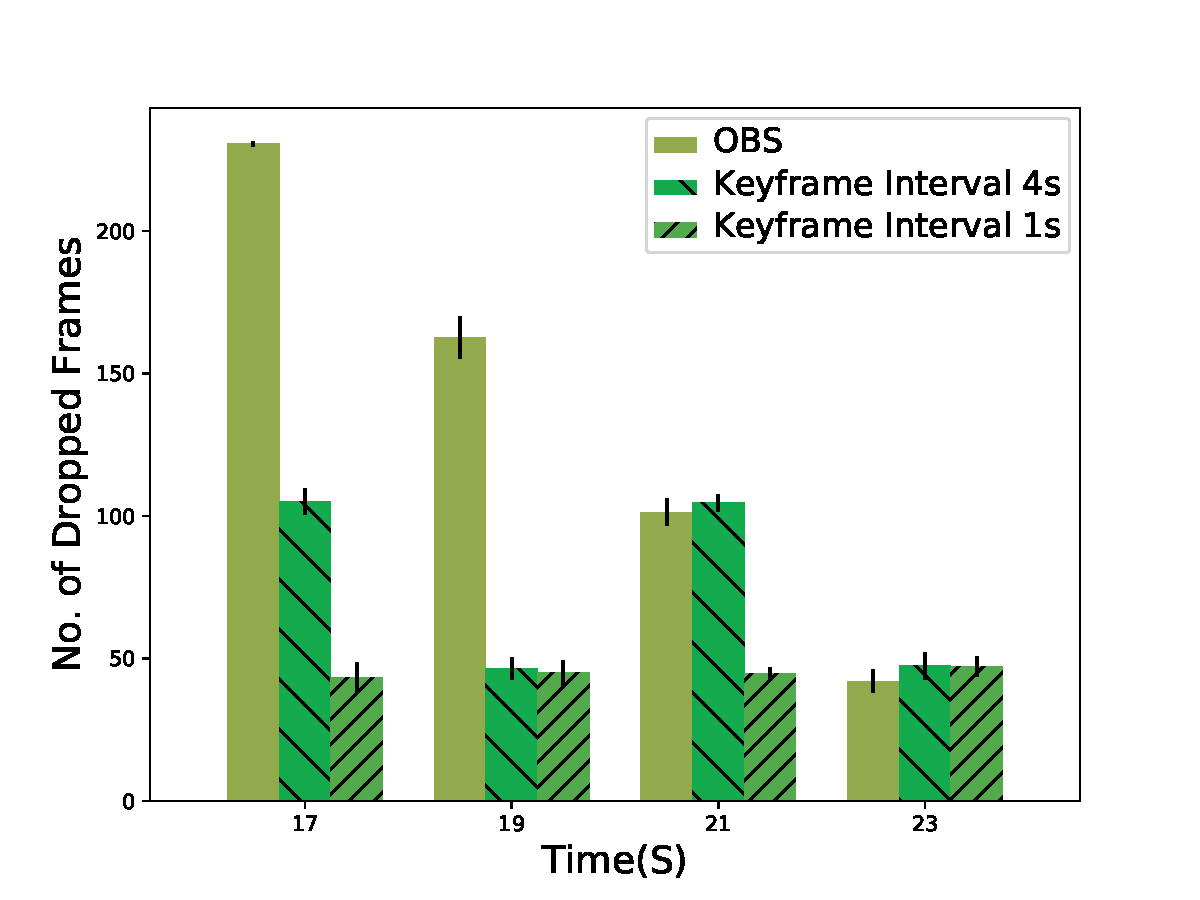
\includegraphics[width=\textwidth]{fig/eval_IframeInterval_drop.pdf}
\caption{Frame drop with varying I frame interval}
\label{fig:iframe-drop}\mylabel{fig:iframe-drop}
\end{subfigure}

\iffalse
\minipage{0.32\textwidth}
  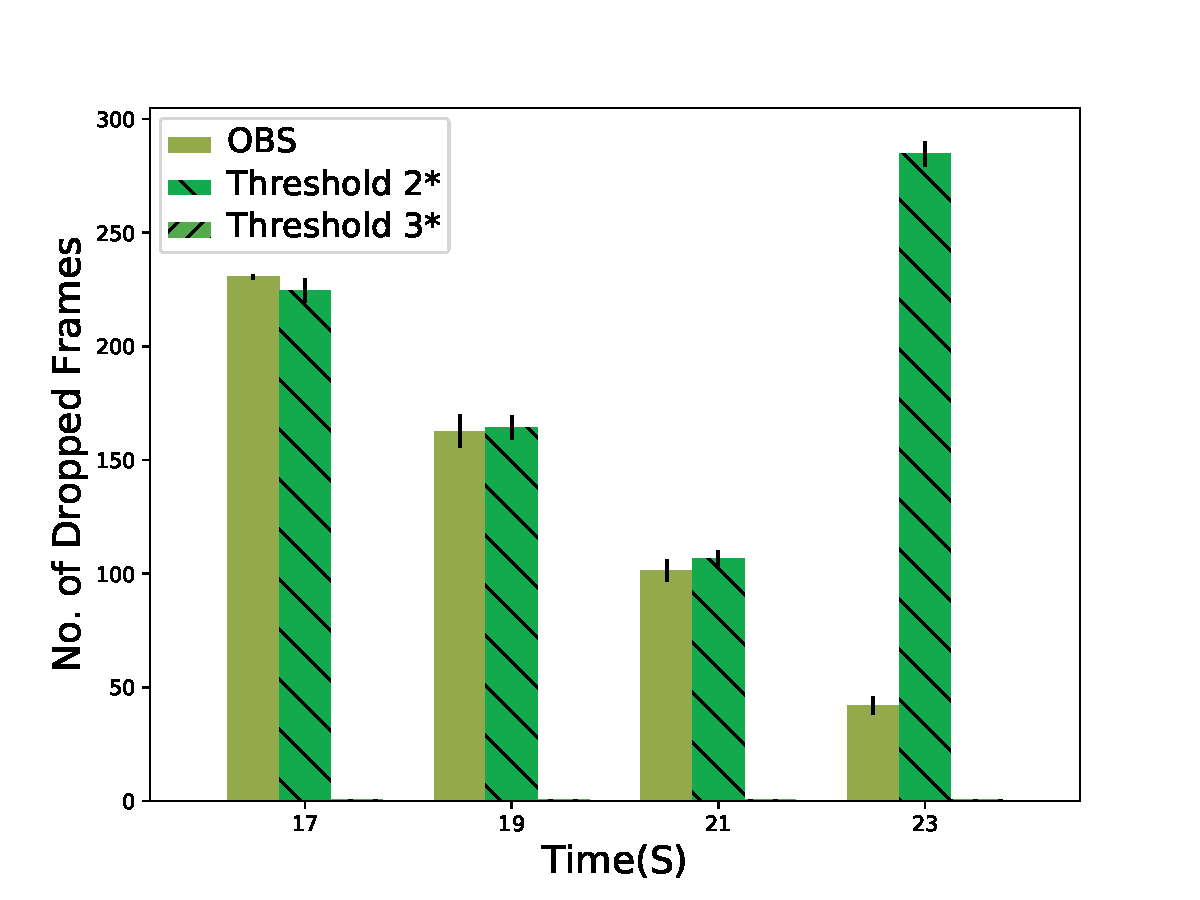
\includegraphics[width=\linewidth]{fig/eval_threshold_drop.pdf}
  \caption{Frame drop with varying threshold}
  \label{fig:threshold-drop}\mylabel{fig:threshold-drop}
\endminipage\hfill
\minipage{0.32\textwidth}
  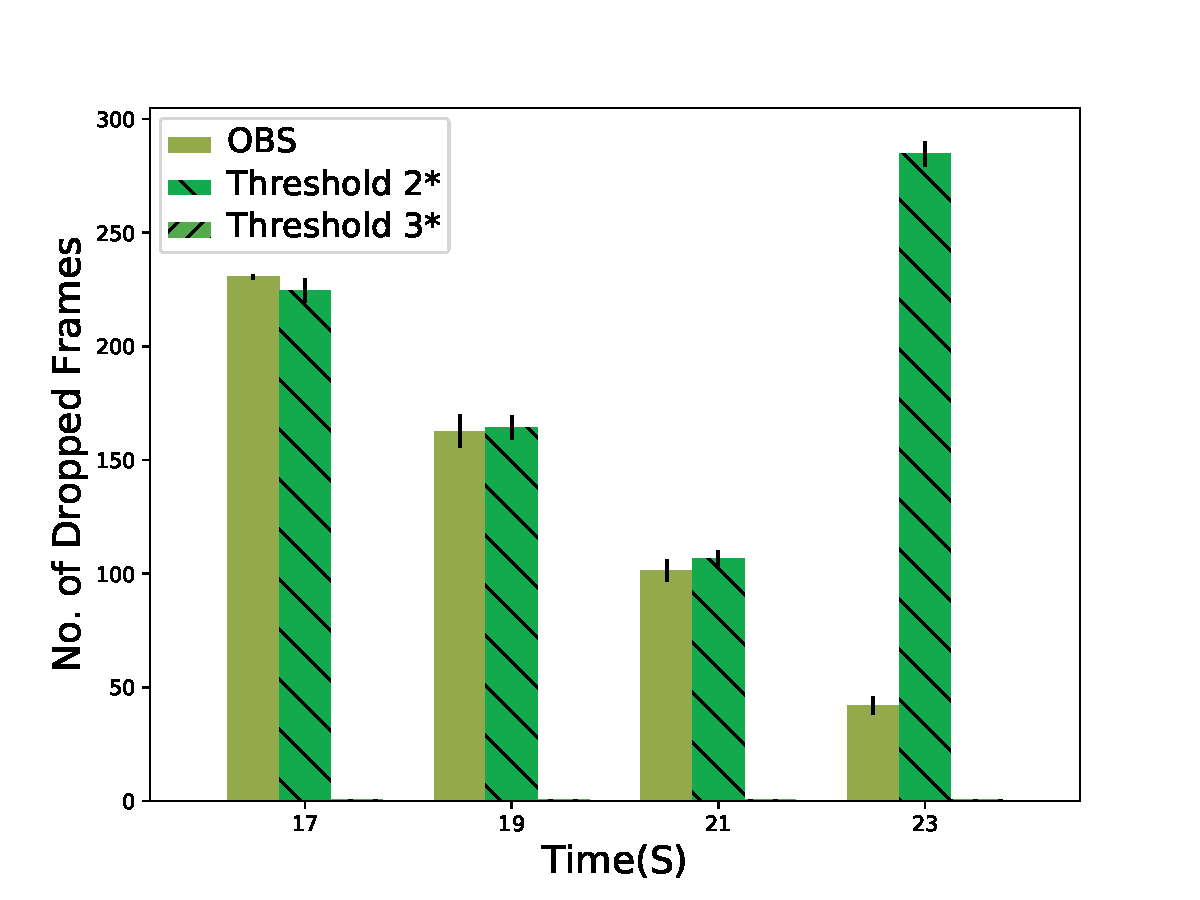
\includegraphics[width=\linewidth]{fig/eval_threshold_drop.pdf}
  \caption{Timeliness with varying I frame interval}
  \label{fig:iframe-timeliness}\mylabel{fig:iframe-timeliness}
\endminipage
\fi

\end{figure}

\iffalse
\begin{figure}
\centering
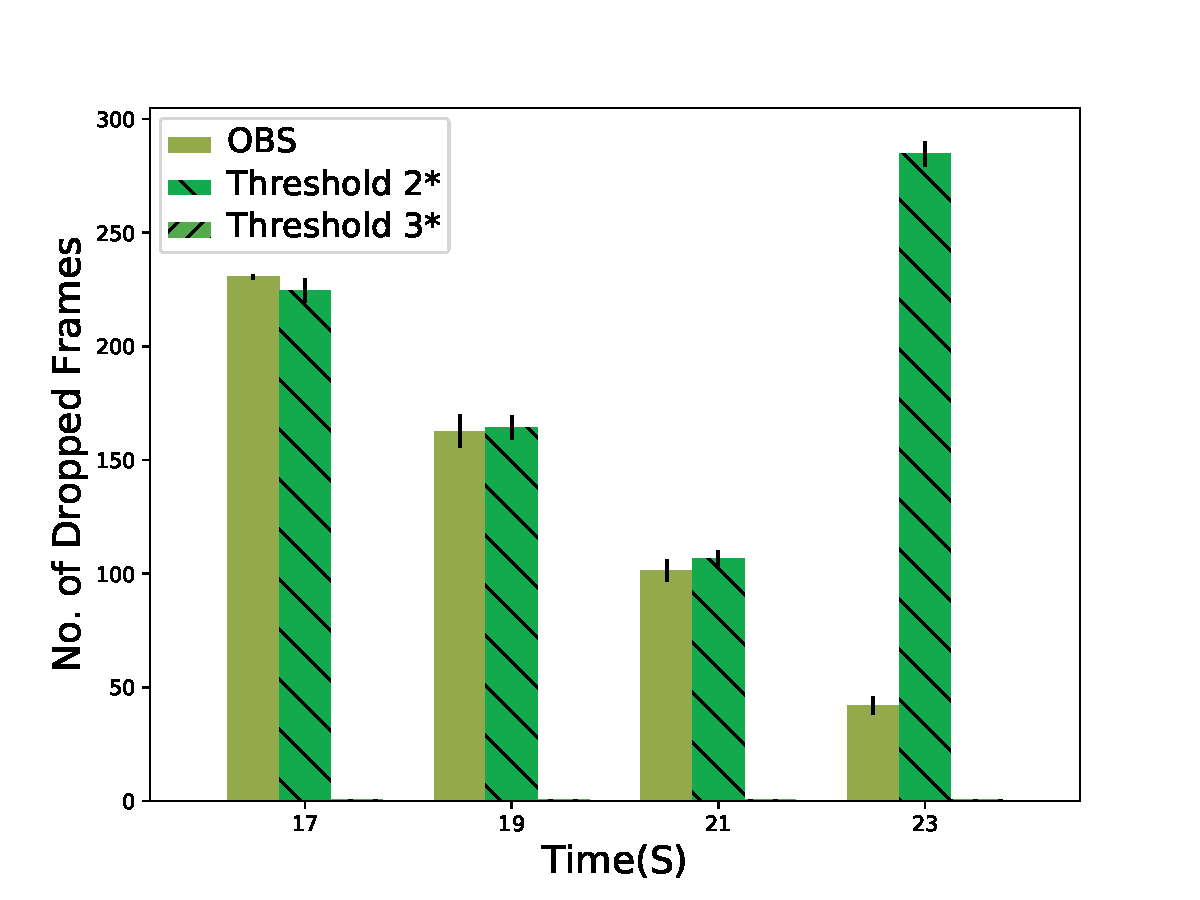
\includegraphics[width=0.32\textwidth]{fig/eval_threshold_drop.pdf}
\caption{Timeliness with varying threshold}
\label{fig:threshold-timeliness}\mylabel{fig:threshold-timeliness}
\end{figure}
\fi 
\textbf{Varying keyframe interval.} The default I frame interval of OBS is 8 seconds, and we adjust it to 4s and 1s in experiments. The frame drops are shown in Figure~\ref{fig:iframe-drop}. We can observe that in each individual experiment, when the interruption starts earlier in a GOP, more frames are dropped. Because an early frame has more following frames depending on it. For default setting, 8 second keyframe interval, when interruption starts at 17s, 19s, 21s, and 23s, the number of frame drops is 238, 164, 105, and 48.
\iffalse
Also, the number of frame drop appears to have the same period with the keyframe interval (e.g., when keyframe interval is 4s, the number of frame drops is 102, 47, 103, and 48 when interruption starts at 17s, 19s, 21s, and 23s, demonstrating a period of 4s.).
\fi
Comparing bars within the group of 17s, we find that smaller keyframe interval significantly reduces the number of frame drop (i.e., from 238, to 102, and 46 when the interval is from 8s to 4s and 1s). However, this reduction is not significant for the group of 23s, because 23s is near the end of a GOP in all cases (8s, 4s, and 1s interval), and there are less frames depending on the frame at 23s.

This experiment shows that if we can eliminate the dependency between frames, an occasional network jitter would only affect frames within a limited duration near the jitter, instead of cascadingly affecting frames in following several seconds.

Reducing keyframe interval is an intractable issue because that adjusting would cause video quality degradation.

\textbf{Video quality and GOP} As mentioned above, the size of GOP needs a tradeoff between video quality and frame dropping. To guide the choice of keyframe interval, we try to vary the GOP and encode many uncompressed streaming using the x264 encoder \cite{x264}. A truth is that the x264 encoder use the delta intermode coding. Thus a larger GOP is much more likely to introduce the accumulative errors, and GOP is recommended smaller than 250 frames. Nevertheless how to determine the specific value is still sophisticated. The video dataset we use contains SD content, HD content, gaming, and 4k content in variety \cite{video_dataset}. The relationship between normalized SSIM and GOP size is displayed in Fig~\ref{fig:ssim_gop}.
We pick four from many videos to represent the result. From the figure, we can see when the GOP size is larger than 0.5s, the SSIM keeps almost the same, with few changes. Additionally combining the previous two experiments, a GOP size larger than 0.5s can achieve better video quality; and a smaller GOP size will reduce the frame dropping. We can see that GOP size between $[0.5,2]$s is probably the best choice for keyframe interval.

\iffalse
\begin{table}[htb]
\centering
\caption{No. of Dropped Frames}
\label{tab:bitrate}\mylabel{tab:bitrate}

\begin{tabular}{|l|l|l|l|l|}
\hline
Bitrate(kbps)          & 1000  & 1500  & 2000  & 2500  \\ \hline
Average Dropped Frames & 148.2 & 148.2 & 149.0 & 150.6 \\ \hline
\end{tabular}
\end{table}
\textbf{Varying bitrate.}
To make the conclusion more visible, we fix keyframe interval to be 8s and introduce network interruption between 19s and 21s. In different experiments, we provide sufficient network bandwidth and vary the bitrate to be 1000kbps, 1500kbps, 2000kbps, and 2500kbps. The frame drop is shown in Table~\ref{tab:bitrate}. The different bitrates do not make much difference, the number of drop in all cases is about 149.

\textbf{Summary.} We summarize and get conclusions. First, reducing keyframe interval leads to less frame drop. Second, bitrate does not influence frame drop for the short-term case, but the quality of each picture. Preliminary Evaluation points out that a small GOP is one useful try.
\fi

\vspace{-0.05in}
\subsection{Greedy Drop Strategy}
To measure the performance, we compare the performance with two algorithms, there are Oracle, Default OBS. Oracle, the offline optimal solution by the brute-force search, which has an exponential time complexity. We pick out one part from the dataset, and the trace lasts for $30$ seconds. During the period both long-term and short period bandwidth fluctuating appears. The keyframe interval is chosen bwteen [0.5,2]s, 1s.

\begin{table}[tb]
\centering
\caption{The Reduction of Frame Drops Normalized to Default OBS}
\label{tab_drop}
{\setlength{\tabcolsep}{1pt}
\begin{tabular}{|c|c|l|}
\hline
\textbf{Algorithm} &\textbf{Play Failure(s)} & \textbf{Percentage}    \\ \hline
Oracle    &265    &$80\%$           \\ \hline
GreedyDrop  &274  &$85.6\%$              \\ \hline
\end{tabular}}
\vspace{-0.1in}
\end{table}

\begin{figure}[htb]
\centering
\begin{subfigure}[b]{.45\columnwidth}
\centering
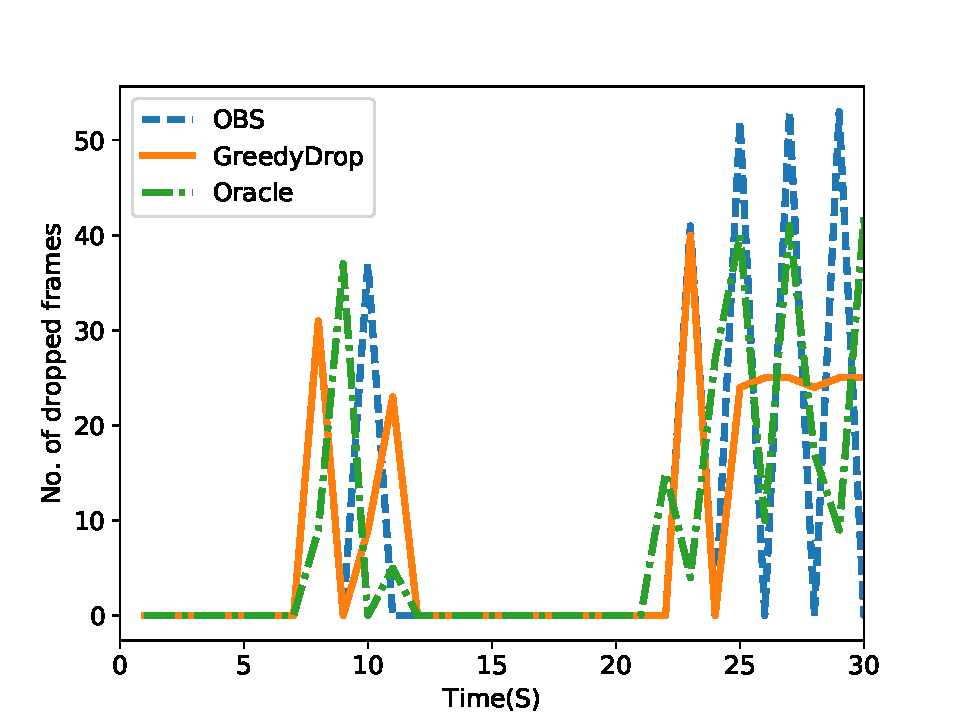
\includegraphics[width=\linewidth]{fig/drop-buffer.pdf}
\caption{No. of frame drop}
\label{fig:drop-buffer}\mylabel{fig:drop-buffer}
\end{subfigure}
\begin{subfigure}[b]{.45\columnwidth}
\centering
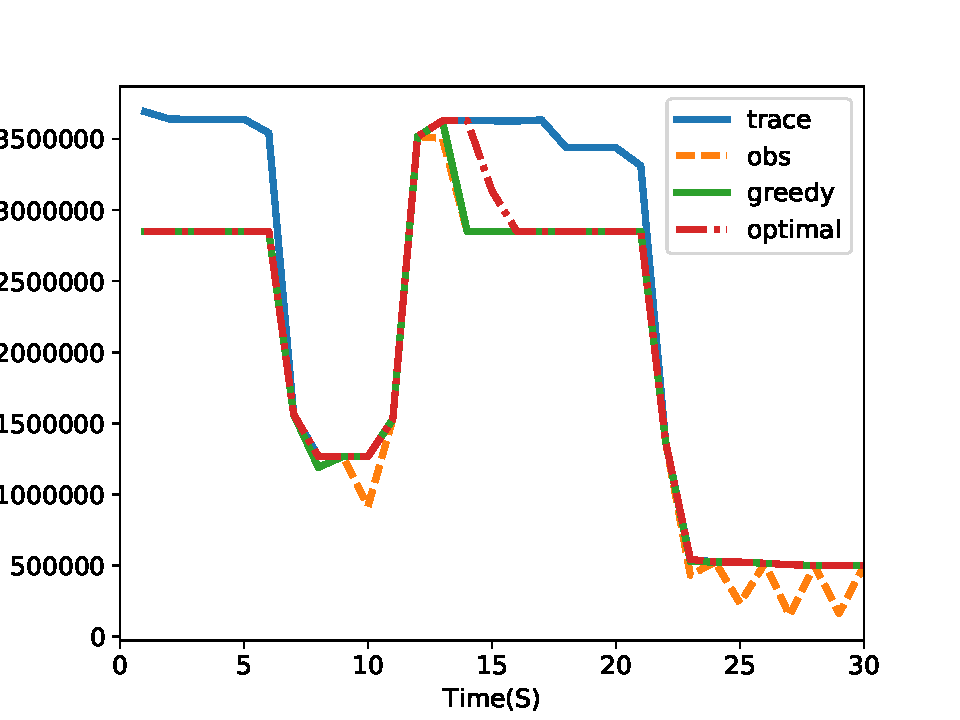
\includegraphics[width=\linewidth]{fig/drop-bandwidth.pdf}
\caption{Real-time throughput}
\label{fig:drop-bandwidth}\mylabel{fig:drop-bandwidth}
\end{subfigure}
\caption{Comparison of different frame drop strategy}
\vspace{-0.15in}
\end{figure} 
The reduction of frame drops is displayed in the table~\ref{tab_drop}. OBS dropped the most frames among three, and GreedyDrop reduce $15\%$, which is a prominent improvement. Morever the gap between GreedyDrop and Oracle is small, less than $5\%$. The frame drop and throughput is shown in Figures~\ref{fig:drop-buffer}~\ref{fig:drop-bandwidth}. The main period of frame dropping locates in 5-10s and 20-30s. All three algorithms perform similarly in 5-10s, but the Oracle will save more frames before the network recovers, and keep a high bandwidth at 10-15s. The frame drop of OBS waves at a high variance in 20-30s, but GreedyDrop almost keeps unchanged. Because GreedyDrop only drops the undecodable frames of the first GOP. For each GOP, the beginning is sent to receiver, and the rest ones is dropped, so for each time, the frame drops and the throughput keep still. Oracle also fluctuates, but with a small variance. Considering both time complexity and performance, GreedyDrop is a good choice.


\subsection{Greedy Adaptive Bitrate}
\begin{figure*}[htb]
\minipage{0.32\textwidth}
  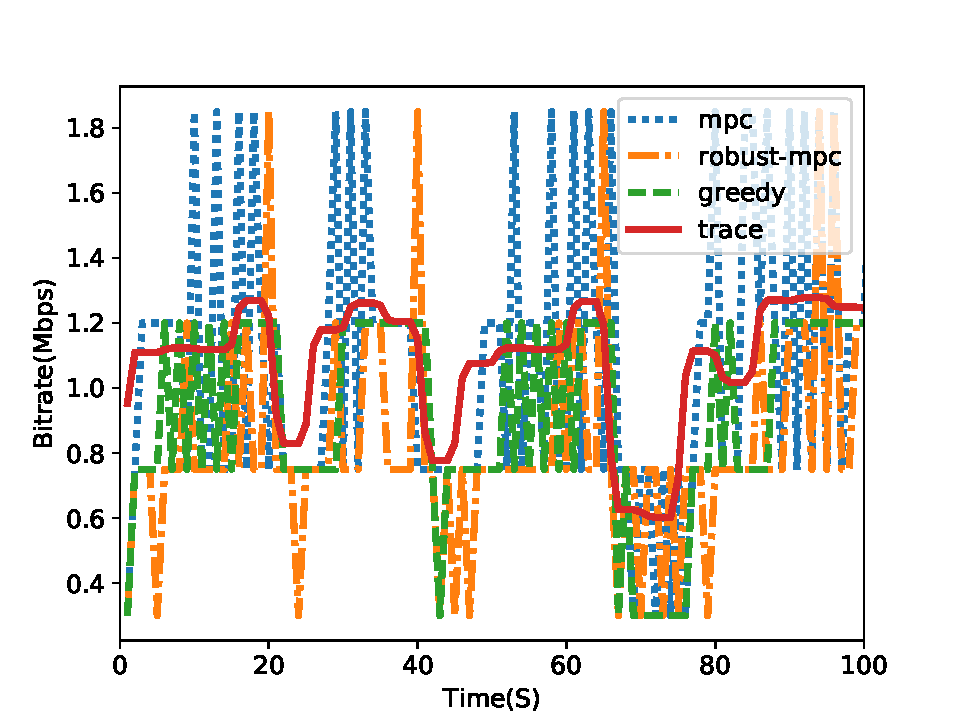
\includegraphics[width=\linewidth]{fig/specific_fcc.pdf}
  \caption{Throughput of FCC dataset}
  \vspace{-0.23in}
  \label{fig:fcc_specific}\mylabel{fig:fcc_specific}
\endminipage
\hfill
\minipage{0.32\textwidth}
  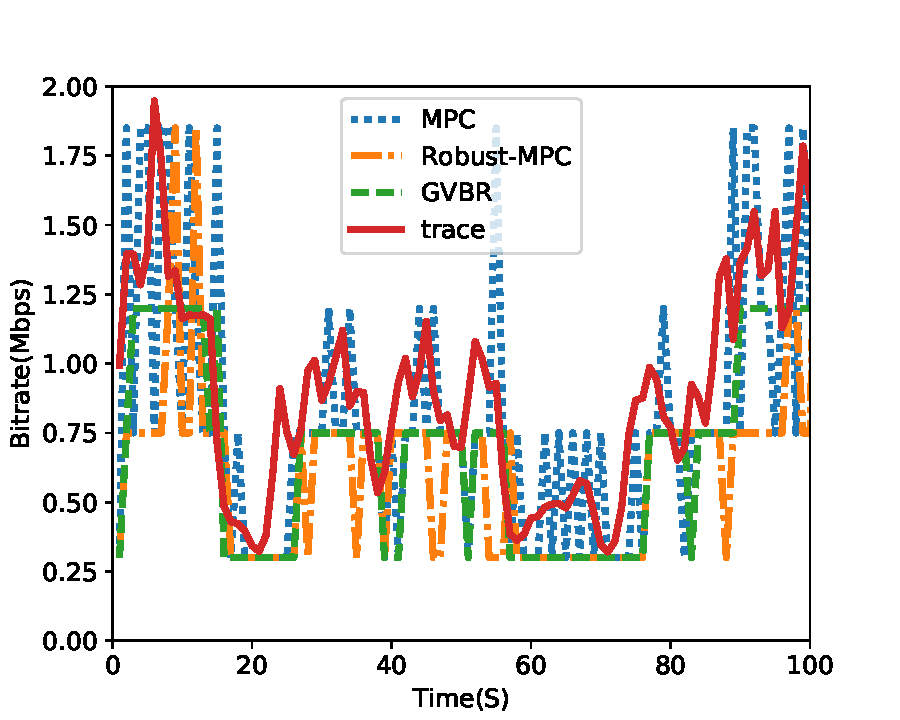
\includegraphics[width=\linewidth]{fig/specific_hsdpa.pdf}
  \caption{Throughput of HSDPA dataset}
  \vspace{-0.23in}
  \label{fig:specific_hsdpa}\mylabel{fig:specific_hsdpa}
\endminipage
\hfill
\minipage{0.32\textwidth}
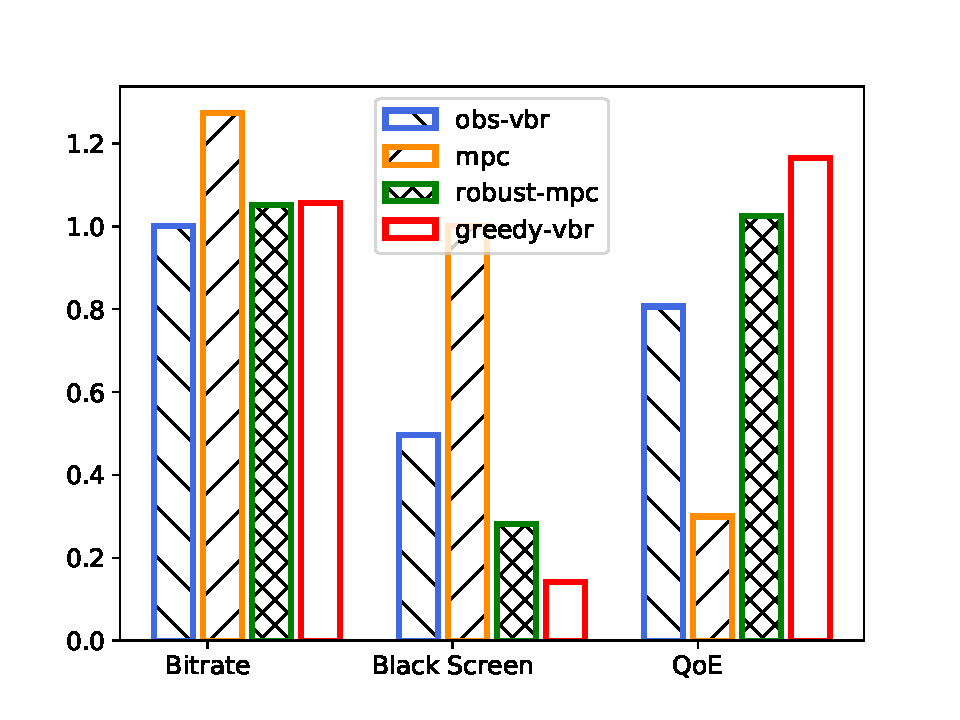
\includegraphics[width=\textwidth]{fig/massive_qoe.pdf}
\caption{Normalized bitrate, play failure and QoE}
\vspace{-0.23in}
\label{fig:vbr-qoe}\mylabel{fig:vbr-qoe}
\endminipage
\end{figure*}

\begin{figure*}[htb]
\minipage{0.32\textwidth}
  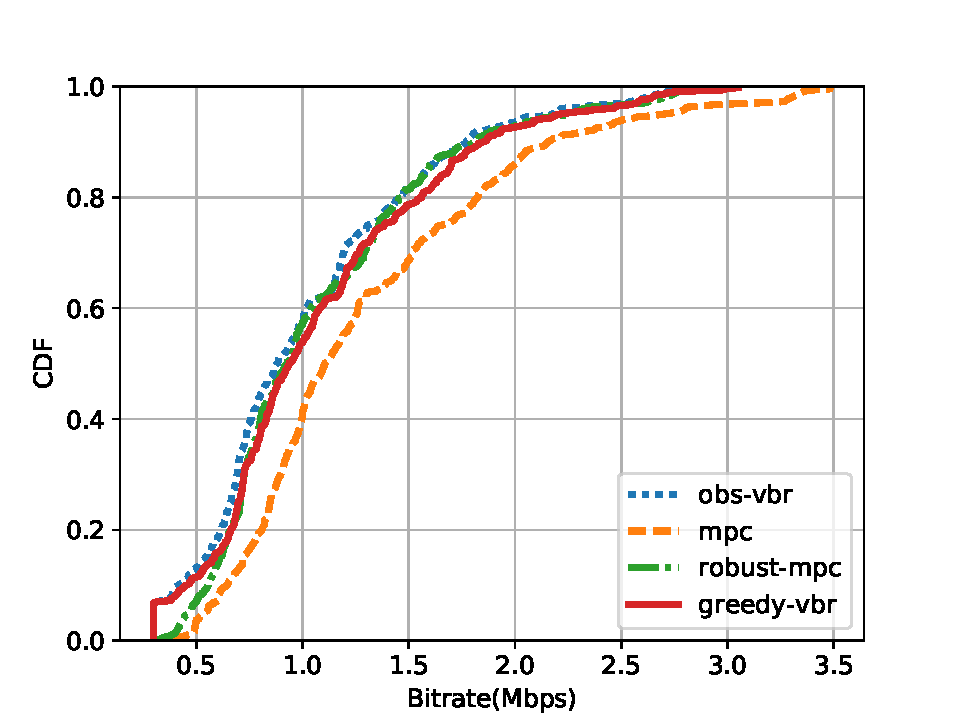
\includegraphics[width=\linewidth]{fig/massive-bitrate-cdf.pdf}
  \caption{CDF of Bitrate}
  \vspace{-0.25in}
  \label{fig:vbr-bitrate-cdf}\mylabel{fig:vbr-bitrate-cdf}
\endminipage
\minipage{0.32\textwidth}
  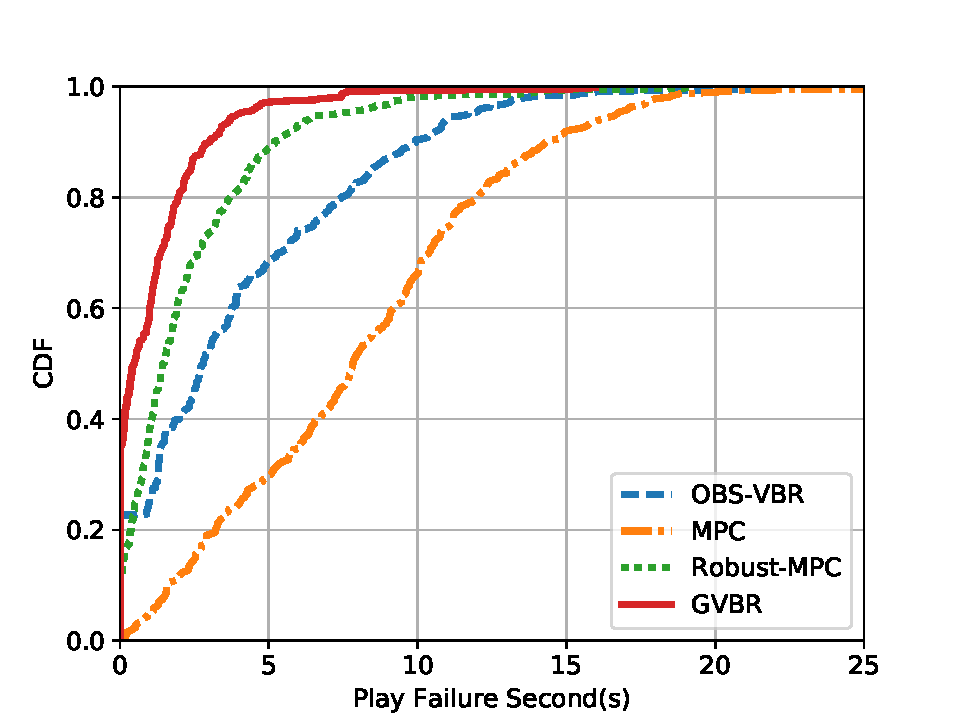
\includegraphics[width=\linewidth]{fig/massive-drop-cdf.pdf}
  \caption{CDF of Play Failure Seconds}
  \vspace{-0.25in}
  \label{fig:vbr-drop-cdf}\mylabel{fig:vbr-drop-cdf}
\endminipage
\minipage{0.32\textwidth}
  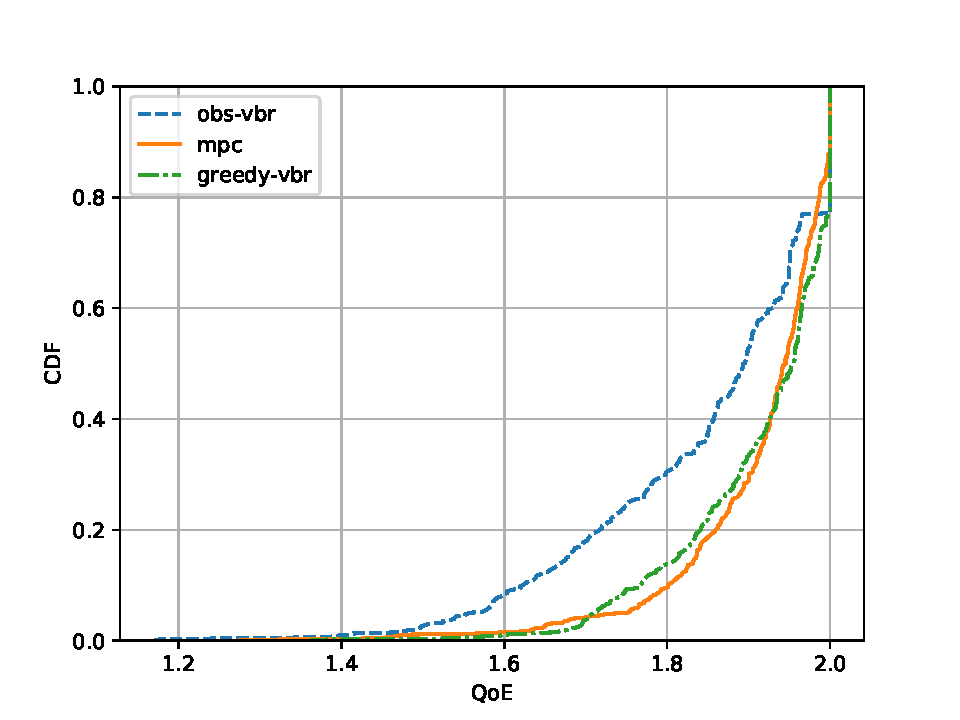
\includegraphics[width=\linewidth]{fig/massive-qoe-cdf.pdf}
  \caption{CDF of Normalized QoE }
  \vspace{-0.25in}
  \label{fig:vbr-qoe-cdf}\mylabel{fig:vbr-qoe-cdf}
\endminipage
\end{figure*} 
We compared GVBR algorihtm towards three algorithms which work excellently in VOD bitrate adaptation, harmonic mean is used for bandwidth estimation:
\begin{itemize}
  \item OBS-VBR: A simple but popular adaptation method. Each time it chooses the bitrate exactly lower than the estimated bandwidth. In addition, use the default drop strategy in OBS.
  \item MPC: use buffer state(number and size of frames, and type of frames, I/P/B) and bandwidth predictions to calculate the optimal bitrate operation in future several time slots. Use the first bitrate choice in next time slot.
  \item Robust-MPC: use the approach resembling MPC, but correct the estimated bandwidth by considering the prediction error in past several time slots.
\end{itemize}
GreedyDrop is adopted as drop strategy(excluding OBS-VBR). Robust-MPC is the state-of-art video adaptation algorithm. The MPC theory can also be applied to live streaming scenario.
Detailed comparison results are shown in Figures ~\ref{fig:fcc_specific} and \ref{fig:specific_hsdpa}. In these two figures, the real line is one real-world trace. Without predication error, MPC prefers to choose higher bitrate than Robust-MPC. Additionally, these two MPC algorihtm always fluctuate around the real bandwidth. In both cases, the MPC and Robust-MPC switch bitrate more frequently than GVBR. Because GVBR tends to choose the lower bitrate than the throughput, when the small bandwidth fluctuation happens, GVBR is less likely to shake. But MPC struggles to achieve the optimal utility, and when the bandwidth increases slightly, MPC has the potential to choose a higher bitrate to maximize the first item in \ref{vbr-formulation}.

A massive simulation is displayed in Figure \ref{fig:vbr-qoe}. We use the combined dataset, FCC and HSDPA to evaluate GVBR algorithm. Normalized QoE is calculated in the figure. Among all, MPC has the maximum bitrate QoE, because the bandwidth estimation is aggressive and MPC has the potential to choose higher bitrate. Three others reach almost the same average bitrate, with little difference, but GVBR is a little higher. With higher bitrate, MPC also drops the most frames, and the time of play failure is the longest. GVBR reduces the play failure to a small value, 50\% reduction compared with Robust-MPC. With higher bitrate and lower play failure, GVBR definitely preforms the best, with the highest QoE.

CDF figures about bitrate, play failure and normalized QoE is as follows, Figure \ref{fig:vbr-bitrate-cdf}, \ref{fig:vbr-drop-cdf}, \ref{fig:vbr-qoe-cdf}. In \ref{fig:vbr-bitrate-cdf}, GVBR lies in the right of Robust-MPC and OBS, with a higher bitrate. $98\%$ of the paly failure is less than 5s in GVBR, about 40\% play fluently with no failure. Only 2\% of GVBR receives poor QoE, the rest 98\% has a high QoE falling in [0.8,1].

The total frame drops compared with original OBS are reduced by 96\%. The play failure time of original OBS method with constant bitrate is 26s in average, and GVBR has a one-second play failure time.

As all, our solution, GVBR achieves a higher bitrate, and at the same time reduces the play failure significantly.


\section{Related Work}
Recently abundant works shed light on seamlessly bitrate adaptation. Most of them are mainly based on DASH, which is called dynamic adaptive streaming over http. All the VBR algorithms in DASH can be classified into several categories: rate-based, buffer-based and the combination of both two. Rate-based methods often pick the highest available bitrate lower than the estimated bandwidth \cite{jiang2014improving}, while buffer-based algorithms choose the bitrate according to the buffer level. If the buffer level is high, it prefers a higher bitrate. However at a low buffer level, a lower bitrate is chosed \cite{huang2003adaptive}. Control theory is also applied to the bitrate adaptation, called MPC. MPC forecasts the future network bandwidth of several slots, and finds the optimal solution during these periods, then applies the first choice \cite{yin2015control}. MPC uses the combination of buffer and throughput. With a large solution space, MPC preforms better than all others.

The difference between DASH and video adaptation in live streaming is the following aspects. The first is, the time granularity, in DASH, the time slot lasts for $2$-$10$ seconds, but in live streaming, the time slot lasts for less than $2$ seconds. The second is, the buffer size, DASH is mainly used in VOD, the buffer usually equals to dozens of seconds, but in live streaming, the buffer almost is less than $1$ second. Most important, all of these are at the viewer's side, while researches about the broadcaster's side is little.

There are also some papers about video adaptation in live streaming scenario. \cite{pires2014dash} includes the idea of adaptive streaming in live streaming, but its focus is how to implement in a massive scale and the challenge mainly lies in the resource management. Another paper also researches low-latency live streaming using DASH \cite{bouzakaria2014overhead}, All these papers talk little about the video transmission quality. \cite{de2011feedback} proposes QAC to switch the encoding parameter using feedback control theory, which is a little hard to implement in practice though.

\section{Conclusion and Future Work}
In the future, we would first implement and test individual design methods in Section~\ref{sec:design-space}, including adaptive GOP selection and online frame drop strategy. In our expectation, the final solution would be a combination of these design methods. For example, increase queue threshold, selectively drop frames if the threshold is reached, and when the network recovers, pick a recent frame, recompute the GOP, and send the timely frames to the network. 



%\nocite{*}
%\section*{Acknowledgments}

\bibliographystyle{abbrv}
\begin{small}
\bibliography{paper}
\end{small}
\label{last-page}

\end{document}

